\documentclass[11pt,a4paper]{article}
\usepackage[utf8]{inputenc}
\usepackage[czech]{babel}
\usepackage[T1]{fontenc}
\usepackage{amsmath}
\usepackage{amsfonts}
\usepackage{amssymb}
\usepackage{graphicx}
\usepackage[a4paper,left=2.5cm,right=1.5cm,top=2.5cm,bottom=3cm]{geometry}
\usepackage{anyfontsize}
\usepackage{float}
\usepackage[absolute, overlay]{textpos}
\usepackage{fancyhdr}
\usepackage[hidelinks]{hyperref}
\usepackage{titlesec}
\usepackage{setspace}
\usepackage{fancyhdr} 
\usepackage[hang, flushmargin, bottom]{footmisc} 
\usepackage{tocloft}
\usepackage{listings}
\usepackage{color}
\usepackage{dirtree} 
\usepackage{etoolbox}

\titleclass{\subsubsubsection}{straight}[\subsection]

\newcounter{subsubsubsection}
\renewcommand\thesubsubsubsection{\thesubsubsection.\arabic{subsubsubsection}}
\renewcommand\theparagraph{\thesubsubsubsection.\arabic{paragraph}} 

\titleformat{\subsubsubsection}
  {\normalfont\normalsize\bfseries}{\thesubsubsubsection}{1em}{}
\titlespacing*{\subsubsubsection}
{0pt}{3.25ex plus 1ex minus .2ex}{1.5ex plus .2ex}

\makeatletter
\renewcommand\paragraph{\@startsection{paragraph}{5}{\z@}%
  {3.25ex \@plus1ex \@minus.2ex}%
  {-1em}%
  {\normalfont\normalsize\bfseries}}
\renewcommand\subparagraph{\@startsection{subparagraph}{6}{\parindent}%
  {3.25ex \@plus1ex \@minus .2ex}%
  {-1em}%
  {\normalfont\normalsize\bfseries}}
\def\toclevel@subsubsubsection{4}
\def\toclevel@paragraph{5}
\def\toclevel@paragraph{6}
\def\l@subsubsubsection{\@dottedtocline{4}{7em}{4em}}
\def\l@paragraph{\@dottedtocline{5}{10em}{5em}}
\def\l@subparagraph{\@dottedtocline{6}{14em}{6em}}
\makeatother

\setcounter{secnumdepth}{4}
\setcounter{tocdepth}{4}
\makeatletter
\renewcommand{\@pnumwidth}{1.75em}
\renewcommand{\@tocrmarg}{2.75em}
\makeatother

\setlength{\TPHorizModule}{1mm}
\setlength{\TPVertModule}{1mm}
\setlength{\headheight}{15.2pt}
\setlength{\parskip}{0.1cm}
\setlength{\headheight}{30pt}

\makeatletter
\pretocmd{\section}{\addtocontents{toc}{\protect\addvspace{5\p@}}}{}{}
\pretocmd{\subsection}{\addtocontents{toc}{\protect\addvspace{5\p@}}}{}{}
\pretocmd{\subsubsection}{\addtocontents{toc}{\protect\addvspace{5\p@}}}{}{}
\pretocmd{\subsubsubsection}{\addtocontents{toc}{\protect\addvspace{5\p@}}}{}{}
\makeatother

\PassOptionsToPackage{hyphens}{url}\usepackage[hidelinks]{hyperref}
\renewcommand{\UrlBreaks}{\do\/\do\0\do\1\do\2\do\3\do\4\do\5\do\6\do\7\do\8\do\9\do\a\do\b\do\c\do\d\do\e\do\f\do\g\do\h\do\i\do\j\do\k\do\l\do\m\do\n\do\o\do\p\do\q\do\r\do\s\do\t\do\u\do\v\do\w\do\x\do\y\do\z\do\A\do\B\do\C\do\D\do\E\do\F\do\G\do\H\do\I\do\J\do\K\do\L\do\M\do\N\do\O\do\P\do\Q\do\R\do\S\do\T\do\U\do\V\do\W\do\X\do\Y\do\Z\do\-\do\_}

\definecolor{grey}{RGB}{229, 228, 226}
\def\excleq{\buildrel!\over=}

\pagestyle{fancyplain}
\fancyhf{}
\chead{\fancyplain{}{Návrh databáze technologií využívajících obnovitelné zdroje energie pro drobné investory}}
\rhead{\fancyplain{}{\thepage}}

\author{Veronika Maurerová}
\title{Návrh databáze technologií využívajících obnovitelné zdroje energie pro drobné investory}
\begin{document}
\thispagestyle{empty}
\vspace*{1cm}
\begin{center}

\includegraphics[scale=1]{lev}\\
\vspace*{1cm}
{\fontsize{25}{25}\textbf{Návrh databáze}}\\
\vspace{0.3cm}
{\fontsize{25}{25}\textbf{technologií využívajících obnovitelné zdroje energie pro drobné investory}}\\
\vspace{2cm}
{\noindent\fontsize{25}{25} \selectfont Bakalářská práce}\\
\vspace*{2cm}
\begin{large}
\textbf{Vypracovala:} Veronika Maurerová\\
\vspace{0.3cm}
\textbf{Vedoucí práce:} Ing. Luboš Nobilis\\
\end{large}
\vspace{7cm}
\begin{large}
České vysoké učení technické v~Praze\\
Fakulta elektrotechnická\\
Softwarové technologie a management - Manažerská informatika
\end{large}

\vspace{1cm}

2014
\end{center}
\newpage

\thispagestyle{empty}
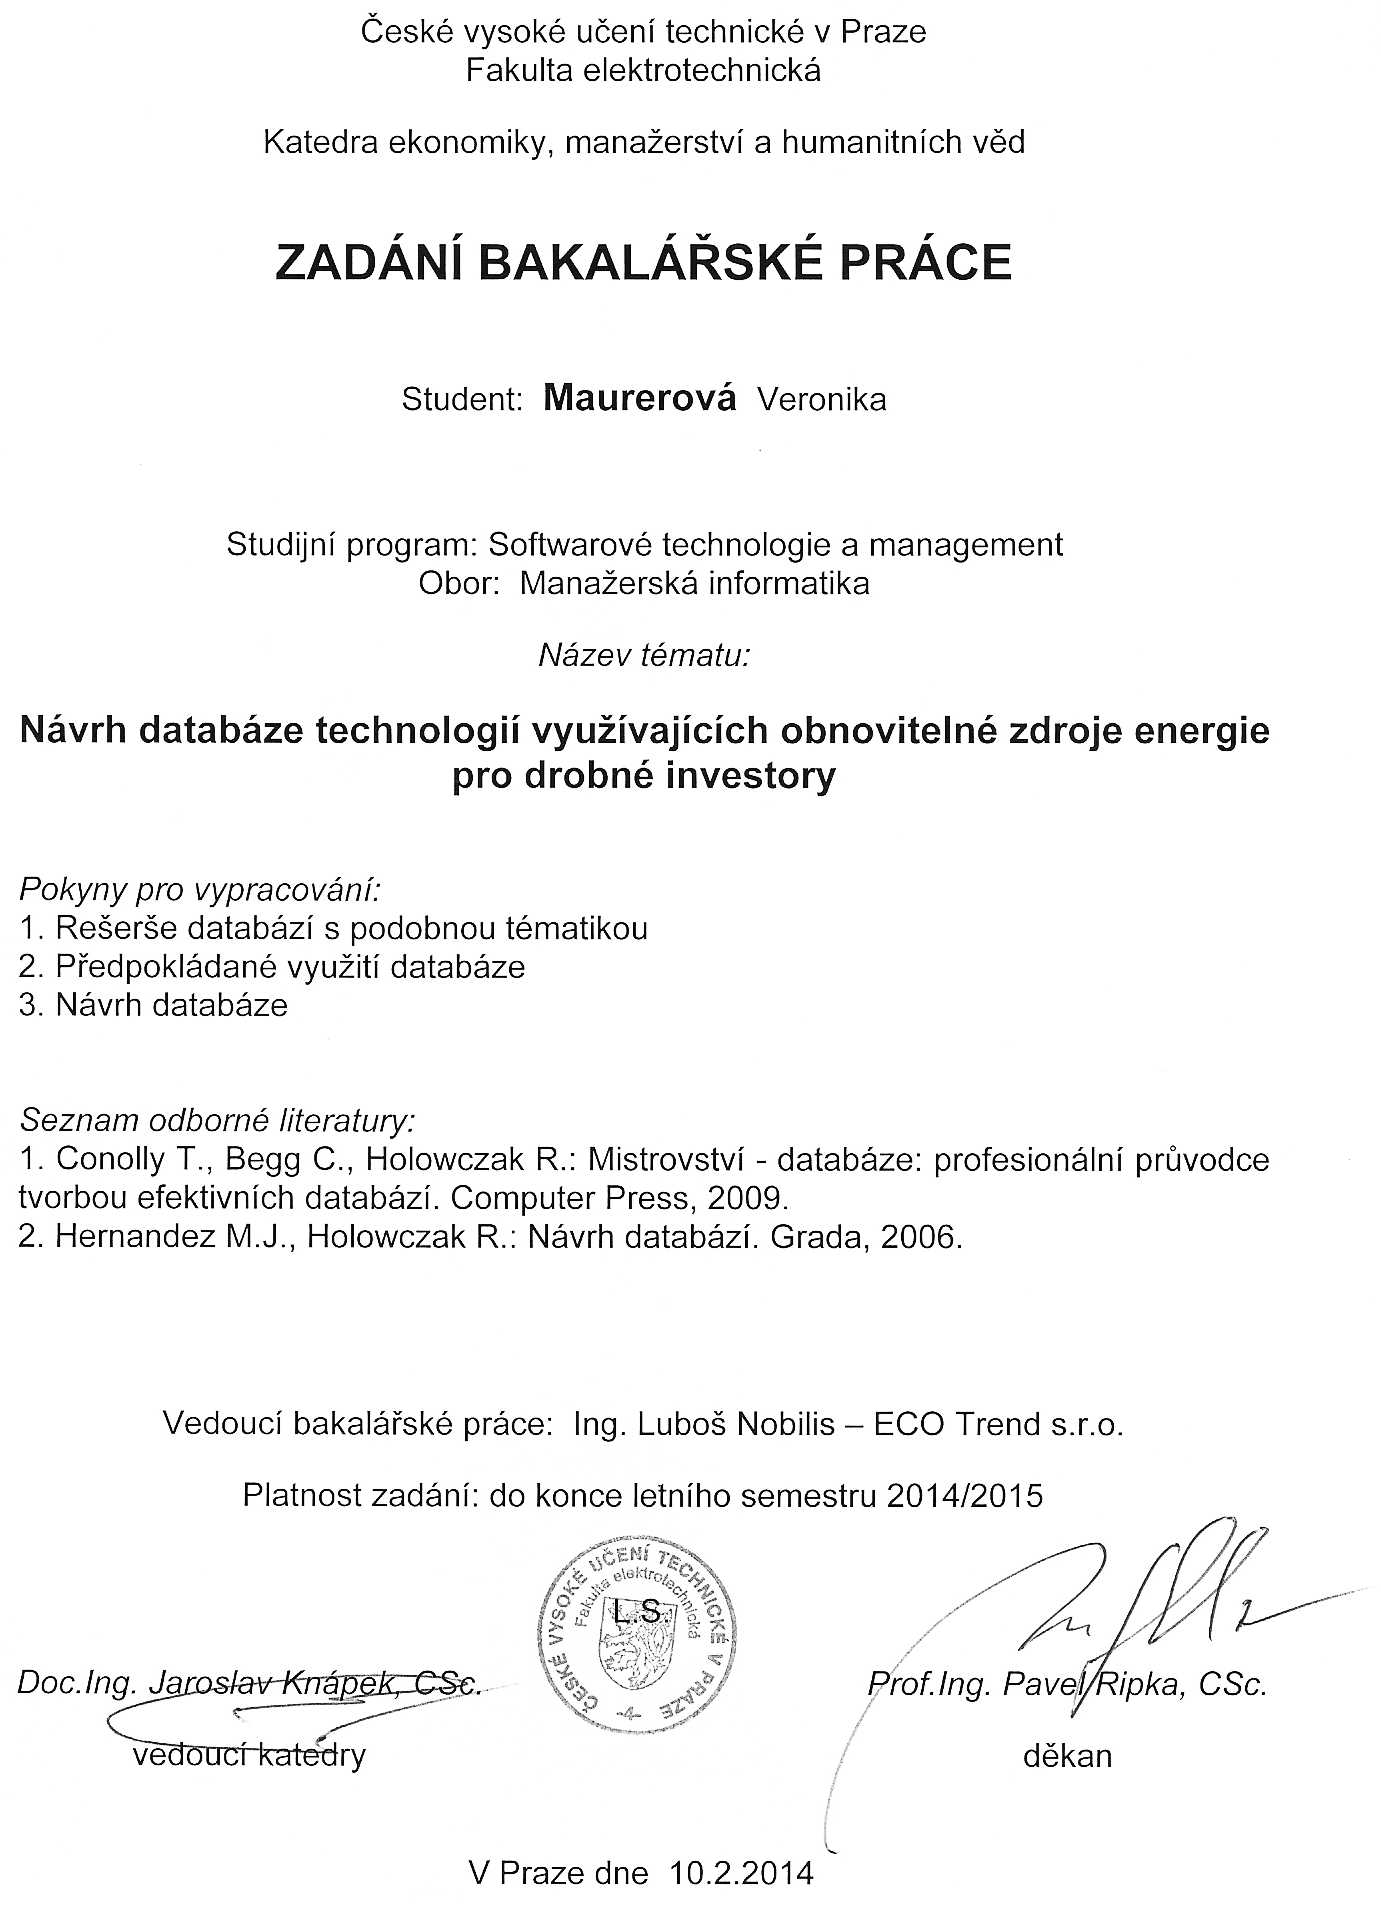
\includegraphics[scale=0.9]{zadani}
\newpage

\thispagestyle{empty}
\vspace*{20cm}
{\Huge \noindent \textbf{Poděkování}}
\vspace{1cm}

\begin{large}
\noindent Děkuji Ing. Luboši Nobilisovi za vedení této práce a dále Ing. Martinu Benešovi, Ph.D. za~konzultace v~rámci katedry. Další poděkování patří
rodině, přátelům a všem těm, kteří mě ve~snaze práci dokončit podpořili.
\end{large}
\newpage

\thispagestyle{empty}
\vspace*{13.5cm}
{\Huge \noindent \textbf{Prohlášení}}
\vspace{1cm}

\begin{large}
 \noindent Prohlašuji, že jsem předloženou práci vypracovala samostatně a že jsem uvedla veškeré použité informační zdroje v souladu s Metodickým pokynem o etické přípravě vysokoškolských závěrečných prací.

Beru na vědomí, že se na práci vztahují práva a povinnosti vyplývající ze zákona č.~121/2000 Sb., autorského zákona, ve znění pozdějších předpisů. V souladu s ust.~§~46 odst.~6 tohoto zákona tímto uděluji nevýhradní oprávnění (licenci) k užití této práce, a to včetně všech příloh, jež jsou její součástí (dále souhrnně jen „Dílo“), a to všem osobám, které si přejí Dílo užít. Tyto osoby jsou oprávněny Dílo užít jakýmkoli způsobem, který nesnižuje hodnotu Díla a za~jakýmkoli účelem (včetně užití k~výdělečným účelům). Toto oprávnění je časově, teritoriálně i~množstevně neomezené.

\vspace{2cm}

\noindent Dne 22. května 2014 v Praze \hspace{8cm} ..................................
\end{large}
\newpage

\thispagestyle{empty}
\vspace*{16cm}
\begin{large}
\noindent České vysoké učení technické v Praze\\
Fakulta elektrotechnická\\
\copyright~2014 Veronika Maurerová. Všechna práva vyhrazena.\\
\textit{Tato práce vznikla jako školní dílo na Českém vysokém učení technickém v Praze, Fakultě elektrotechnické. Práce je chráněna právními předpisy a mezinárodními úmluvami o právu autorském a právech souvisejících s právem autorským. K jejímu užití, s výjimkou bezúplatných zákonných licencí, je nezbytný souhlas autora.}\\
\end{large}

\vspace{0.5cm}
\thispagestyle{empty}
{\huge \noindent \textbf{Odkaz na tuto práci}}
\vspace*{1cm}

\noindent MAUREROVÁ, Veronika. \textit{Návrh databáze technologií využívajících obnovitelné zdroje energie pro drobné investory}. Praha, 2014. Bakalářská práce. České vysoké učení technické v Praze, Fakulta elektrotechnická. Vedoucí práce Ing. Luboš Nobilis. 

\newpage
\thispagestyle{empty}
\vspace*{5cm}
{\Huge \noindent \textbf{Abstrakt}}
\vspace*{1cm} 

\noindent Tato bakalářská práce řeší návrh databáze dle konkrétního zadání. Zadáním je databáze technologií využívajících obnovitelné zdroje energie pro drobné investory. Práce je reakcí na poptávku firmy ECO~trend~s.r.o. Cílem práce je prozkoumat dosavadní situaci v oblasti dostupných databází na podobné téma, uspořádat požadavky na danou funkční aplikaci, na základě těchto požadavků popsat metodiku návrhu relační databáze a navrhnout konkrétní databázi. V rámci požadavků na databázi jsem se zaměřila především na jejich formulaci. Součástí požadavků je i návrh rozhodovacího formuláře, který hodnotí potenciální investice do produktů uložených v databázi. V rámci návrhu formuláře zvažuji vhodné metody hodnocení investic. Při návrhu jsem se zaměřila na konceptuální, logický i fyzický návrh konkrétní relační databáze. Hlavním výsledkem této práce je dokumentace jak požadavků, tak návrhu databáze pro konkrétní aplikaci, a dále skript k vytvoření databáze na databázovém serveru.\\  

\noindent \textbf{Klíčová slova:}\\
\textit{případy užití, hodnocení investice, návrh relační databáze, SQL skript}.

\vspace{1.5cm}

{\Huge \noindent \textbf{Abstract}}
\vspace*{1cm}

\noindent The thesis describes the database design according to the specific assignment, which is to create a database of technologies using renewable energy sources for small investors. The assignment is a reaction on the demand of ECO trend s.r.o. comapny. The aim is to examine the current situation of available databases in a similar fields, list the requirements of the application, describe the methodology of relational database design and propose specific database according to these requirements. In the context of the requirements, I focused mainly on their formulation. One of the requirements is also a draft of a form, which evaluates potential investments in products listed in the database. In a part of this draft I consider suitable methods of evaluation of the investments. In the context of database design, I focused on the conceptual, logical and physical design of a specific relational database. The main result of this work is the documentation of the requirements, database design for the specific application, and the script that may be used to create the database on the database server. \\

\noindent \textbf{Keywords:}\\
\textit{use cases, investment evaluation, relational database design, SQL script}.

\newpage
\tableofcontents
\newpage

\onehalfspacing
\section{Úvod}
Tématem práce je Návrh databáze technologií využívajících obnovitelné zdroje energie pro drobné investory (dále jen DTOZE). Na zadání bakalářské práce se podílela firma ECO trend s. r. o., která specifikovala požadavky na databázi a dodala základní informace o~datech, které mají být v~databázi uloženy. Dále se podílela na specifikování využití databáze.

Databáze, která bude zpřístupněna přes webovou aplikaci, má poskytnout laické i odborné veřejnosti přehled o~technologiích využívajících obnovitelné zdroje energie (dále jen OZE) a především rozsáhlé informace o~konkrétních produktech a jejich producentech či dodavatelích. V databázi by měly být produkty, které jsou dostupné pro drobné investory (např. malé vodní a větrné elektrárny) a~které lze umístit na pozemky či obydlí dostupné pro běžné uživatele elektrické energie či tepla. Tyto informace mají pomoci většímu rozšíření povědomí o využití OZE mezi běžné uživatele především v~České republice. Součástí aplikace budou i další funkčnosti např. pokročilé vyhledávání či formulář který ze~zadaných parametrů navrhne vhodné varianty využití OZE a zhodnotí výhodnost investice. Což má za cíl zlepšit orientaci v datech, ale také nabídnout konkrétní optimální varianty dle možností daného uživatele. 

Cílem práce je prozkoumat současnou situaci v oblasti dostupných databází týkajících se OZE, uspořádat požadavky na danou funkční aplikaci a na základě těchto požadavků popsat metodiku návrhu databáze, jejíž výsledkem bude návrh konkrétní databáze. Cílem práce není vytvořit kompletní aplikaci, ale připravit databázi pro další implementaci.
Chtěla jsem pracovat na projektu, který bude mít reálné využití, proto jsem zvolila po dohodě se zástupcem vedoucího katedry toto téma. Tvorba podobných systémů mě zajímá a zabývám se jí i přesto, že zaměření mého oboru je více ekonomické než softwarové.   

Obsah práce je rozdělen na tři hlavní části. V~první části se zabývám rešerší databází na podobné téma v~odvětví OZE. Nalezené databáze krátce popisuji a zdůrazňuji jejich klady a zápory, popř. v~čem mě inspirovaly. V další části se zabývám využitím databáze, kde zmiňuji požadavky na databázi, popisuji mechanismus vyhledávání a vysvětluji další funkčnosti aplikace, která má na základě návrhu databáze vzniknout. Tato část je nezbytná pro návrh databáze, který popisuji v poslední části. V~poslední nejrozsáhlejší části se zaměřuji na metodiku návrhu databáze. Popisuji jednotlivé fáze návrhu od konceptuálního přes logický až po fyzický návrh a metodiku demonstruji na konkrétním návrhu.  

\newpage
\section{Rešerše databází s~podobnou tématikou}
Rešerše se používá k~hledání vhodných zdrojů informací před zahájením psaní odborné práce.\footnote{Rešerše. \textit{Ústřední knihovna ČVUT} [online]. [cit. 2013-12-10]. Dostupné z: \url{http://knihovna.cvut.cz/sluzby/reserse/co-je-reserse.html}.}  Využila jsem postup rešerše k~vyhledání konkrétních databází, které jsou dostupné na Internetu. Cílem bylo zjistit, zda existují podobné databáze, jak jsou koncipované, jaké mají klady a zápory, zda má vůbec význam takovou databázi vytvářet. Hledala jsem databáze, které obsahují data podobná tématu týkající se OZE.  U nalezených databází jsem hodnotila, jak se týkají konkrétních technologií využívajících OZE, na co se zaměřují, zda jsou přehledné, jak jsou aktuální apod.

\subsection{Postup rešerše}
V~následujících podkapitolách popisuji postup rešerše a bližší seznámení s~databázemi, které jsem pomocí rešerše našla. Postup rešerše jsem čerpala z~interaktivního průvodce na stránkách Knihovny univerzitního kampusu Masarykovy univerzity v~Brně\footnote{Rešerše: modelový příklad postupu. \textit{Správa Univerzitního kampusu Masarykovy Univerzity} [online]. [cit. 2013-12-10]. Dostupné z: \url{http://ukb.muni.cz/kuk/animace/eiz/Reserse/reserse_praxe.html}.}.

\subsubsection{Formulace tématu} 
Základem rešerše je formulovat správně téma, ke kterému hledám informace, v~mém případě konkrétní webové stránky. Není vhodné se omezit pouze na český jazyk, ale je důležité formulovat téma i v~jiných jazycích, minimálně alespoň v~anglickém jazyce. Já zvolila téma následující:\\\\
Téma v~českém jazyce: Databáze technologií využívajících obnovitelné zdroje energie pro drobné investory.\\
Téma v~anglickém jazyce: Database of technologies using renewable energy sources for small investors.

\subsubsection{Definice klíčových slov}
Důležité je si definovat i klíčová slova, jelikož téma je často složité a nelze jej vložit jako celek do vyhledávače.  Samotná klíčová slova však nemusí stačit, a proto je vhodné si stanovit i nadřazená klíčová slova nebo synonyma. Opět vše stanovuji současně i v~angličtině.\\\\
\textbf{Klíčová slova:}\\  
databáze technologií využívajících obnovitelné zdroje energie, database of technologies using renewable energy sources;\\
technologie využívající zdroje energie, technologies using renewable energy sources.\\\\
\textbf{Nadřazená klíčová slova:}\\
databáze obnovitelných zdrojů energie, database of renewable energy sources;\\
databáze OZE, database of RES;\\
obnovitelné zdroje energie, renewable energy sources;\\
zdroje energie, energy sources.\\\\
\textbf{Synonyma:}\\ 
databáze technologií využívajících OZE, database of technologies using RES;\\
databáze technologií využívajících obnovitelné přírodní zdroje energie, database of technologies using natural renewable energy sources;\\
databáze technologií využívajících přírodní nefosilní zdroje energie, database of technologies using natural renewable non-fossil energy sources;\\
katalog technologií využívajících OZE, catalog of technologies using RES.\\

\subsubsection{Vyhledávání}
Až po přípravě vhodných slov a frází lze přejít k~samotnému vyhledávání. K~vyhledávání jsem použila tři vyhledávače: Google.com, Seznam.cz, Bing.com. Zadávala jsem nejdříve klíčová slova a synonyma, ale s~výsledkem jsem nebyla spokojena. Musela jsem použít nadřazená slova. S~nadřazenými slovy jsem již měla více výsledků.  Ze všech výsledků jsem vyhodnotila jako vhodné následující databáze, týkající se obnovitelných zdrojů energie: 
\begin{enumerate}
\item Databáze environmentálních služeb a výrobků, zobrazení subjektů na mapě, podrobnější informace o~subjektech - \url{http://www.envisluzby.cz/}. 
\item Mezinárodní evropská databáze politik v~oblasti OZE - \url{http://www.res-legal.eu/}.
\item Databáze OZE - informace o~jednotlivých druzích OZE, kontakty na subjekty v~ČR zabývající se OZE, kontaktní osoby - \url{http://daze.vukoz.cz/daze/index.jsp}.
\end{enumerate}

\subsection{Vyhodnocení nalezených databází}
Rešerší jsem zjistila, že momentálně není na Internetu dostupná žádná online databáze technologií využívajících obnovitelné zdroje energie (natož pro drobné podnikatele či investory) v~českém nebo anglickém jazyce. Nalezla jsem však několik databází, které jsou po obsahové stránce podobné – zabývají se tématem obnovitelných zdrojů energie. Některé z~nich mě inspirovaly, jiné navedly k jinému řešení.

\subsubsection{Databáze environmentálních služeb a výrobků}
Databázi environmentálních služeb a výrobků provozuje České ekologické manažerské centrum (CEMC).  Databáze vznikla v~rámci tříletého projektu „Důsledky liberalizace environmentálních služeb“, financovaného z~prostředků Grantové agentury České republiky. Databáze vznikla v~roce 2011 a nyní je v~databázi zaregistrováno 1079 subjektů.

Obsahem databáze jsou subjekty, které poskytují služby, vyrábí technologie, výrobky, přípravky, vzdělávají nebo provádějí výzkum za účelem předejít vzniku škody na životním prostředí, zmírnit či odstranit negativní dopad na životní prostředí, zdraví a majetek osob na území České republiky. Do~databáze se subjekty dostávají přes registraci, která je zdarma. Uvedou základní údaje o~firmě a~výpis služeb či výrobků, které nabízejí. 

Na webových stránkách lze zobrazit seznam všech subjektů, v~kterém lze hledat podle typu služeb, dle zpracovatelů odpadů nebo dle názvu subjektu. Vedle seznamu jsou subjekty zaznamenány i~v~mapě se štítkem, který specifikuje zaměření firmy. Mapu lze přibližovat a oddalovat, popř. lze vybrat konkrétní kraj, okres či město. Lze zobrazit detail subjektu, kde jsou zobrazeny kontaktní údaje a na co se subjekt zaměřuje.\footnote{Envisluzby.cz. CEMC. \textit{Databáze enviromentálních služeb a výrobků} [online]. 2011 [cit. 2013-12-10]. Dostupné z: \url{http://www.envisluzby.cz/}.}

\subsubsection{RES LEGAL Europe}
RES LEGAL Europe databáze byla vytvořena z~iniciativy Evropské komise. Je to online volně dostupná databáze v~anglickém jazyce, editovaná odborníky. Obsahem databáze jsou informace o~právních předpisech, státních podporách a záležitostech týkající se obnovitelných zdrojů energie ve 27 zemí Evropské unie (dále EU), v~zemích ESVO a některých nových členských zemí EU. Databáze zahrnuje tři energetické odvětví: elektřina, vytápění a chlazení, doprava.

Cílem databáze je poskytnout jednak rychlý přehled o~různých právních předpisech dané země zaměřených na OZE a současně data zobrazit jasně, výstižně a přehledně. Databáze je aktualizována pravidelně. Datum vytvoření a poslední aktualizace, jméno odpovědné osoby a další informace se zobrazují u~každého profilu dané země.
Popisy jsou vytvořeny na základě příslušných zákonných zdrojů. Obsahují i odkazy na původní právní prameny v~původním jazyce. Většinou je k~dispozici i odkaz na překlad zákona. Na stránce je k~dispozici také seznam kontaktů na vnitrostátní orgány a odborníky, které lze dále kontaktovat.

Každá země má na stránkách vlastní profil, na kterém lze dohledat veškeré informace týkající se dané země. Databáze umožňuje srovnávat jednotlivé země na základě státních podpor, záležitostí týkající se silových elektrických a komunikačních sítí a politik a předpisů. Dále lze na stránkách vyhledávat pomocí srovnávacího nástroje, který umožní vybrat země, typ energetického sektoru a další specializace daného sektoru a zobrazit požadované informace v~tabulce. Lze si i prohlédnout archiv dokumentů seřazený dle zemí. Tato databáze je velmi přehledná i přes její rozsáhlost. Zaměřuje se však pouze na administrativní záležitosti ohledně OZE.\footnote{Res-legal.eu. EUROPEAN COMISSION. \textit{Renewable energy policy database and support} [online]. 2012 [cit. 2013-12-10]. Dostupné z: \url{http://www.res-legal.eu/}.}

\subsubsection{DAZE}
Databáze obnovitelných zdrojů energie DAZE shromažďuje informace o~obnovitelných zdrojích energie. V~první části obsahuje seznam firem, které se zabývají OZE, v~další části se pak blíže zaměřuje na biomasu. Vznikla a vyvíjela se za finanční podpory výzkumného projektu „Zdokonalování stávajících technologií využívání obnovitelných zdrojů a úspor energie“~(MŽP ČR 320/3/99), projektu „Vyšší využití nepotravinářské zemědělské produkce v~průmyslu“~(MZe ČR QF 4142) a projektu „Nepotravinářské využití biomasy v~energetice“~(MŠMT 2B06131).  

Z~databáze lze získat profily jednotlivých firem. Ty obsahují název firmy, adresu, webové stránky, popř. kontaktní osobu. Lze pak zobrazit i všechny kontaktní osoby obsažené v~databázi a zobrazit si též jejich profil s~kontaktními údaji. Seznamy jsou seřazené podle abecedy.  Subjekty lze vyhledávat i~dle zaměření na konkrétní typ OZE. 

V~druhé části lze získat velmi podrobné informace o~plodinách, které jsou vhodné pro produkci biomasy. Ty jsou opět v~seznamu seřazeném podle abecedy, lze však zobrazit i~seznamy dle typu plodiny (např. bioplyn, brikety, vrby, topoly, atd.). Každá plodina má vlastní profil, kde jsou zobrazeny informace o~typu plodiny, v~jakých lokalitách ji lze pěstovat, jaké lze očekávat výnosy, jak se pěstuje, možnosti využití a mnoho dalšího. Informace jsou členěny do záložek. Ze stránek lze tisknout data dané plodiny, stáhnout soubor ve formátu PDF nebo zobrazit ve formátu XML. 

Tato databáze se nejvíce podobá zadání DTOZE. Obsahuje strukturovaná data a profily jednotlivých subjektů a druhů OZE, i když specializovaných pouze na biomasu. Je určená pro odbornou i laickou veřejnost. DAZE je vytvářena a průběžně aktualizována pracovníky odd. fytoenergetiky VÚKOZ Průhonice ve spolupráci s~dalšími organizacemi.\footnote{Daze.vukoz.cz. VÝZKUMNÝ ÚSTAV SILVA TAROUCY PRO KRAJINU A~OKRASNÉ ZAHRADNICTVÍ, veřejná výzkumná instituce. \textit{DAZE: Databáze obnovitelných zdrojů energie} [online]. 2005 [cit. 2013-12-10]. Dostupné z: \url{http://daze.vukoz.cz/daze/index.jsp}.}

\newpage

\section{Předpokládané využití databáze}
Před samotným návrhem databáze pro aplikační software (zkráceně aplikaci) je důležité si projít i~předcházející fáze životního cyklu vývoje databáze, kterými jsou plánování databáze, definice systému a~sběr a~analýza požadavků.\footnote{CONOLLY, Thomas, Carolyn BEGG a Richard HOLOWCZAK. Mistrovství - databáze: profesionální průvodce tvorbou efektivních databází. Vyd. 1. Brno: Computer Press, 2009, 584 s. ISBN 978-80-251-2328-7. Str. 109.} 

Informace z těchto fází se netýkají pouze samotné databáze (tedy ukládání a zpřístupnění dat), ale celého systému, který bude nad databází fungovat. Na sběru těchto informací se podílí zadavatel a vývojář (pokud se jedná o menší systém). V případě větších či složitějších systémů jsou do vstupní analýzy zahrnuti i budoucí uživatelé systému (např. zaměstnanci firmy či samotní zákazníci) a z řad vývojářů i několik analytiků, kteří používají různé metody zjišťování požadavků. Zjištěné informace je klíčové sepsat a potvrdit oběma stranami. Ujasní se tak veškeré požadavky a podmínky obou stran. Takový dokument se nazývá vize projektu. Vize projektu DTOZE vznikala souběžně s vypracováním tohoto textu a je přílohou \ref{attach:DTOZE-vize}.   

Pro návrh databáze je klíčové si se zadavatelem ujasnit požadavky a jednotlivé případy užití, jelikož z těchto dat se vychází při návrhu celého systému. Proto neuvádím celou vizi jakou součást textu této práce, ale pouze její část. Definici systému, funkční a obecné požadavky a specifikování funkčnosti formuláře popisují následující kapitoly. Při analýze a popisu požadavků jsem vycházela z~knihy Mistrovství databáze\footnote{Tamtéž str. 109 - 153.} a spolupracovala se zaměstnanci firmy ECO trend. Metodiku analýzy a sběru dat podrobně nerozepisuji, jelikož není předmětem této práce. Podrobněji se věnuji pouze vysvětlení funkčnosti formuláře (v kapitole č.~\ref{cap:specifikovani_funkcnosti_formulare}), který je na základě požadavků nutné sestavit a~rozhodnout se pro vhodné výpočty a~správné metody hledání. 

\subsection{Definice systému} 
Cílem DTOZE je zpřístupnit široké veřejnosti metodiku rozvoje drobných OZE bez veřejné podpory na internetu přes webovou aplikaci. Informace budou zpřístupněny přes webovou aplikaci především  přes katalog produktů, které pro výrobu elektrické energie využívají OZE. Pomocí aplikace bude možné získat doporučení pro jaký produkt se rozhodnout či další informace o OZE či jednotlivých technologiích využívajících OZE.

\subsection{Funkční požadavky na systém}
Funkční požadavky na systém lze rozdělit do tří základních modulů:

\begin{itemize}
\item katalog produktů:
\begin{itemize}
\item zobrazení detailu produktu,
\item vícekriteriální vyhledávání,
\item administrace katalogu,
\end{itemize}
\item interaktivní formulář:
\begin{itemize}
\item vyhledání nejvhodnějších produktů dle zadání,
\item výpočet efektivnosti investice,
\end{itemize}
\item obecné informace o OZE a technologiích využívajících OZE.
\end{itemize}

Podrobnější popis a konkrétní zpracování jsou uvedeny v jednotlivých pohledech. Pohled popisuje stručně požadavky, které byly sjednány. Dále jsou zobrazeny v diagramu jednotlivé případy užití, které byly vytvořeny na základě požadavků. Pro vizualizaci případů užití používám nástroj Enterprise Architect.    

\subsubsection{Pohledy}
Systém bude rozlišovat několik pohledů - pohled běžného uživatel, producenta, administrátora. Pohled běžného uživatele sdílí producent i správce. Pohled producenta je ve většině případů odlišný od pohledu správce a proto nelze označit pohled správce za nadřazený pohledu producenta s přidanou funkčností. Prolínání pohledů znázorňuje obrázek č. \ref{fig:pohledy}.

\begin{figure}[H] 
\centering 
\caption{Prolínání pohledů na DTOZE} 
\vspace{0.1cm}
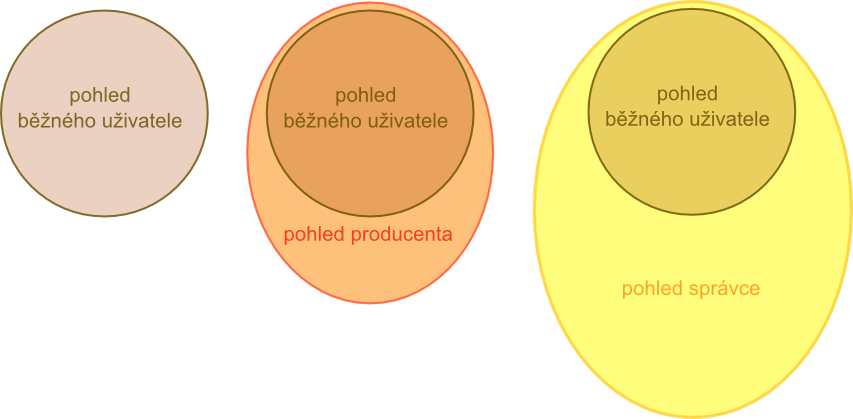
\includegraphics[scale=0.4]{vize_DTOZE_pohledy1} 
\label{fig:pohledy}
\end{figure} 

Jednotlivé možnosti uživatelů v různých pohledech popisují následující podkapitoly. Pod každým pohledem je uveden diagram znázorňující jednotlivé případy užití a vazbu na pohled a dále je uvedena tabulka, která obsahuje případy užití na dle pohledů s popisem. V tabulce je také uvedena obtížnost implementování a priorita vypracování. Popisky k jednotlivým hodnotám jsou znázorněny v tabulce č.~\ref{fig:obtiznost} a tabulce č.~\ref{fig:priorita}.

\begin{table}[H] 
\centering 
\caption{Popisek vysvětlující značené obtížnosti v tabulkách případů užití} 
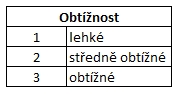
\includegraphics[scale=0.5]{vize_DTOZE_UC_0_obt} 
\label{fig:obtiznost}
\end{table} 

\begin{table}[H] 
\centering 
\caption{Popisky vysvětlující značení priority v tabulkách případů užití} 
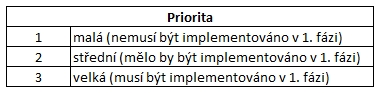
\includegraphics[scale=0.5]{vize_DTOZE_UC_0_prior} 
\label{fig:priorita}
\end{table} 

\subsubsubsection{Pohled běžného uživatele}
Běžný uživatel zobrazí technologie ve všech kategoriích, vyhledává a filtruje v~těchto datech. Dále zobrazí obecné informace k~technologiím či o~výrobci, sleduje základní statistiky, zobrazí informace o~projektu či zadavateli. Může využít filtrovací formulář pro získání doporučení jaké technologie využívající OZE jsou vhodné. Z~běžného uživatele se stane producent (registrovaný uživatel) po vyplnění registrace a schválení registrace správcem. Diagram a tabulka případů užití z pohledu běžného uživatele je znázorněn na obrázku č.~\ref{fig:UC_diagram_BU} (diagram) a v tabulce č.~\ref{fig:UC_tabulka_BU}. 

\begin{figure}[H] 
\centering 
\caption{Diagram případů užití z pohledu běžného uživatele}
\vspace{0.1cm} 
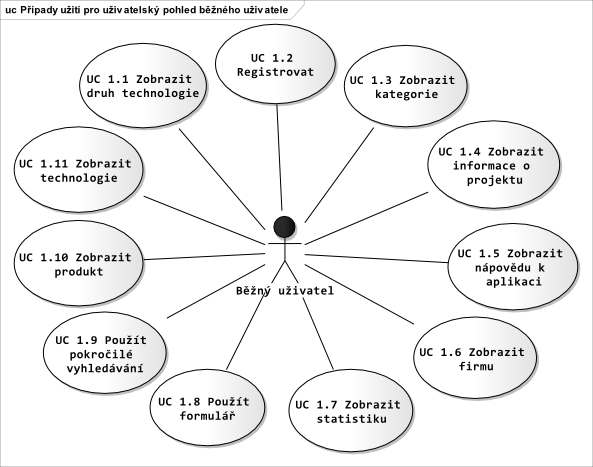
\includegraphics[scale=0.8]{vize_DTOZE_UC_dg1_n} 
\label{fig:UC_diagram_BU}
\end{figure} 

\begin{table}[H] 
\centering 
\caption{Tabulka případů užití z pohledu běžného uživatele} 
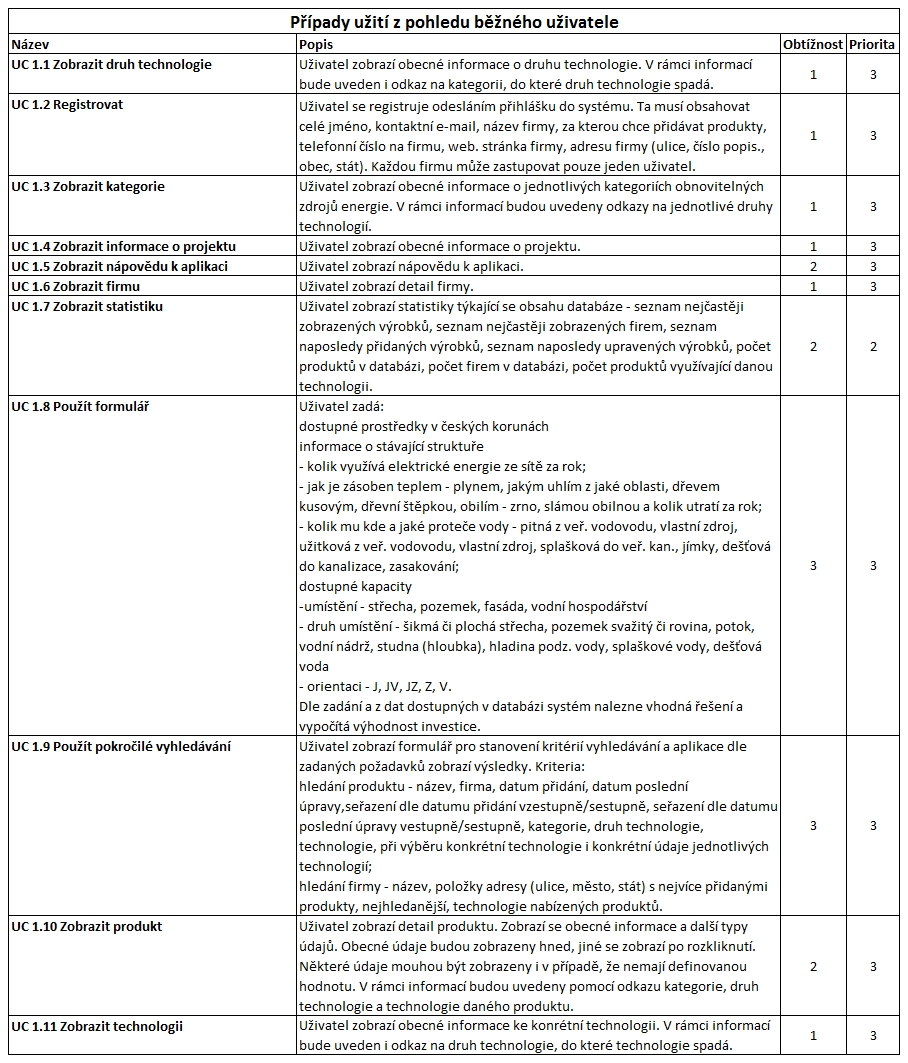
\includegraphics[scale=0.5]{vize_DTOZE_UC_1} 
\label{fig:UC_tabulka_BU}
\end{table} 

\subsubsubsection{Pohled producenta}
Producent může vše co běžný uživatel. Po úspěšné registraci a  přihlášení se může podílet na obsahu databáze. Registrovat se může výrobce či dodavatel produktů a přidávat tak do databáze své výrobky, které vyrábí či dodává a ještě nejsou v~databázi zaznamenané. Může uvést ve svém profilu bližší informace o~své firmě či doplnit chybějící údaje. Na svém profilu může sledovat, kolik záznamů přidal do databáze, které čekají na schválení a které byly zamítnuty. Jeho účet může být deaktivován. Diagram a tabulka případů užití z pohledu producenta je znázorněn na obrázku č. \ref{fig:UC_diagram_S} (diagram) a v tabulce č.~\ref{fig:UC_tabulka_S}. S~pohledem správce producent sdílí dva případy užití, které jsou znázorněny samostatně v tabulce č.~\ref{fig:UC_tabulka_SaA}. 

\begin{figure}[H] 
\centering 
\caption{Diagram případů užití z pohledu producenta} 
\vspace{0.1cm} 
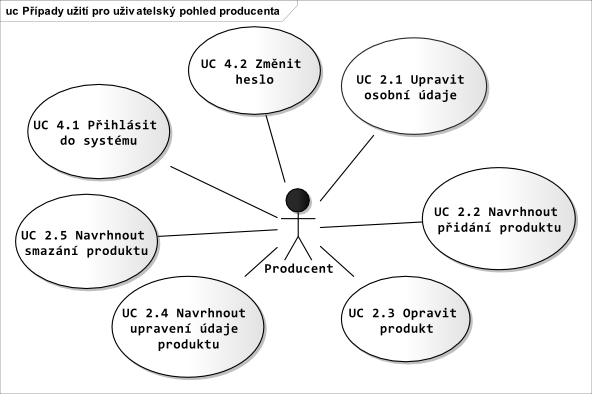
\includegraphics[scale=0.8]{vize_DTOZE_UC_dg2_n} 
\label{fig:UC_diagram_S}
\end{figure} 

\begin{table}[H] 
\centering 
\caption{Tabulka případů užití z pohledu producenta} 
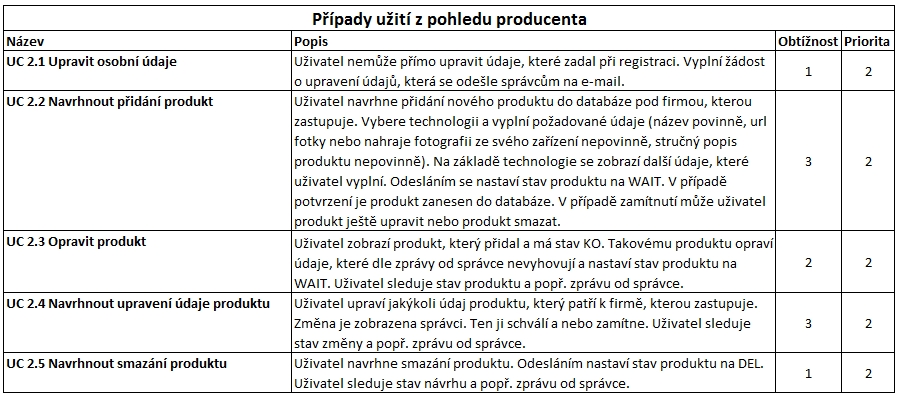
\includegraphics[scale=0.5]{vize_DTOZE_UC_2} 
\label{fig:UC_tabulka_S}
\end{table} 

\subsubsubsection{Pohled správce}
Správce se stará o~veškerý obsah webové aplikace. Přidává produkty do databáze, edituje je nebo maže. Produkty může přidávat manuálně či je importovat. Může editovat obecné informace o~kategoriích a~technologiích, obecné informace o~projektu. Má přístup k~veškerým statistikám. Dále potvrzuje a~ruší přihlášky uživatelů, kteří mají zájem přispívat do databáze. Validuje také nově přidané výrobky a~žádosti o změnu od registrovaných uživatelů. Producentům, kteří nedodržují pravidla pro přidávání nových produktů může správce deaktivovat účet. Také administrátorům může deaktivovat účet. Má možnost vytvořit i nového správce. Dále také může editovat formulář, přidávat nebo mazat dotazníkové položky. Diagram a tabulka případů užití z pohledu správce je znázorněn na obrázku č.~\ref{fig:UC_diagram_A} (diagram) a~v~tabulce č.~\ref{fig:UC_tabulka_A}. S pohledem producenta správce sdílí dva případy užití, které jsou znázorněny samostatně v~tabulce č.~\ref{fig:UC_tabulka_SaA}. 

\begin{figure}[H] 
\centering 
\caption{Diagram případů užití z pohledu správce} 
\vspace{0.1cm} 
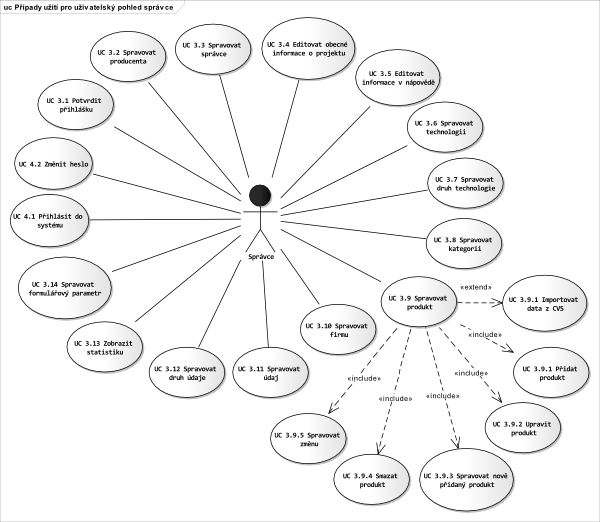
\includegraphics[scale=0.9]{vize_DTOZE_UC_dg3_n} 
\label{fig:UC_diagram_A}
\end{figure} 
 
\begin{table}[H] 
\centering 
\caption{Tabulka případů užití společných pro pohled producenta a správce} 
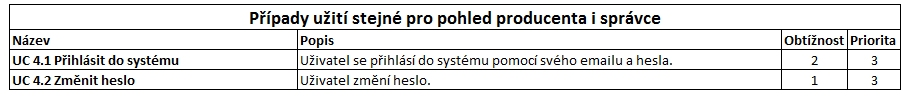
\includegraphics[scale=0.5]{vize_DTOZE_UC_4} 
\label{fig:UC_tabulka_SaA}
\end{table}

\begin{table}[H] 
\centering 
\caption{Tabulka případů užití z pohledu správce} 
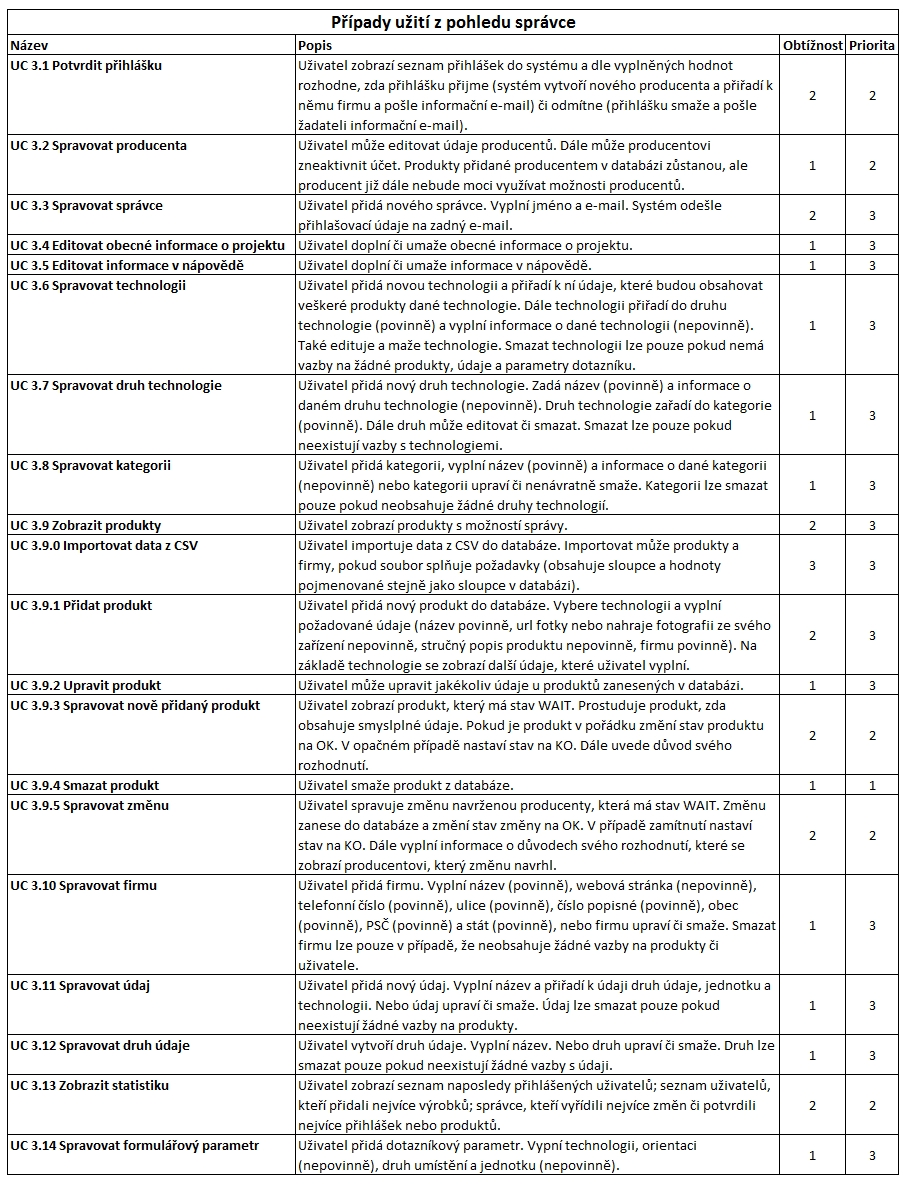
\includegraphics[scale=0.5]{vize_DTOZE_UC_3} 
\label{fig:UC_tabulka_A}
\end{table} 
 
\subsection{Systémové požadavky na databázi}
\subsubsection{Počáteční velikost databáze}
Předpokládá se, že největší nárůst databáze bude ihned po spuštění celého systému. Pověření lidé od~zadavatele již nashromáždili velké množství dat a další shromažďují.  Předpokládanou velikost databáze při zahájení provozu znázorňuje tabulka č. \ref{fig:poc_velikost_databaze}. 

\begin{table}[H] 
\centering 
\caption{Tabulka počáteční velikosti databáze} 
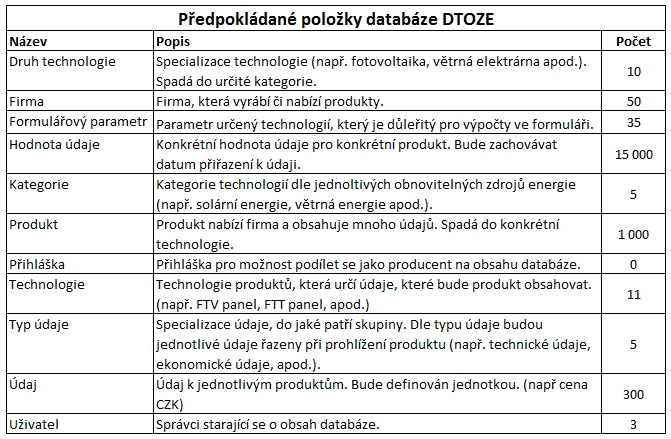
\includegraphics[scale=0.5]{vize_DTOZE_UC_veldata} 
\label{fig:poc_velikost_databaze}
\end{table} 

\subsubsection{Růst velikosti databáze}
Databáze bude růst především v počtu produktů, které budou přidávány. Nepředpokládá se velký nárůst uživatelů ani v obecných položkách jako je např. technologie, kategorie, údaj apod. Předpokládaný růst za měsíc a za rok znázorňuje podrobněji tabulka č \ref{fig:rust_databaze}. 

\begin{table}[H] 
\centering 
\caption{Tabulka předpokládaného růstu za měsíc a za rok} 
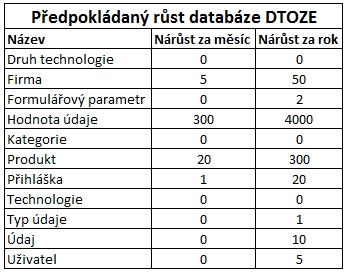
\includegraphics[scale=0.5]{vize_DTOZE_UC_veldatapo} 
\label{fig:rust_databaze}
\end{table} 

\subsubsection{Typy a průměrný počet prohledávaných záznamů}
Předpokládá se, že databázový systém prostřednictvím webové aplikaci navštíví ze začátku 5 lidí denně později až 20 lidí denně. Dle toho se odvíjí i typy a průměrný počet prohledávaných záznamů, které popisuje tabulka č. \ref{fig:zaznamy}.

\begin{table}[H] 
\centering 
\caption{Tabulka typů vyhledávání a průměrný počet prohledávaných záznamů} 
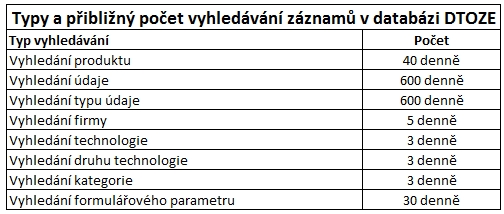
\includegraphics[scale=0.45]{vize_DTOZE_UC_vyhled} 
\label{fig:zaznamy}
\end{table} 

\subsubsection{Výkon}
Očekávaná odezva je méně než 1 sekundu při vyhledávání 1 záznamu.
Očekávaná odezva je méně než 3 sekundy při vyhledávání více záznamů.

\subsubsection{Uživatelské rozhraní}
Uživatelské rozhraní bude mít podobu webové aplikace. Uživatelské rozhraní bude uživatelsky příjemné a bude obsahovat online dostupnou nápovědu pro všechny pohledy. 

\subsubsection{Zabezpečení}
Aplikace bude zpřístupněna pomocí platného e-mailu a hesla. U producentů po potvrzení přihlášky, kde uvedou i údaje o firmě, kterou budou zastupovat. Správci mohou přidělit přístup i dalším osobám pověřeným správou databáze. Uživatelé budou mít práva upravovat obsah databáze dle jednotlivých pohledů (tedy dle pohledu producenta a pohledu správce).

\subsection{Specifikování funkčnosti formuláře}\label{cap:specifikovani_funkcnosti_formulare}
Jednou z funkčností webové aplikace je interaktivní formulář. Tento formulář bude dostupný pro všechny uživatele aplikace. V popisu případů užití je zmíněno co přesně uživatel zadá za data, a~co formulář vyhodnotí za výsledky, ale není konkrétně popsáno, jak bude fungovat. V následujících kapitolách podrobně popisuji jaké výpočty bude aplikace provádět, a s jakými daty krom dat zadaných uživatelem bude tyto výpočty provádět. Jaká data získá od uživatele znázorňují jednotlivé obrázky - na~obrázeku č.~\ref{fig:formular_navrhA} je formulář k~získání informace o dostupných prostředcích, na obrázku č.~\ref{fig:formular_navrhB} je formulář k získání informace o stávajících prostředcích a na obrázku č.~\ref{fig:formular_navrhC} je poslední formulář k získání informace o~dostupných kapacitách. Jedná se pouze o návrh, jednotlivé položky můžou být implementovány různě, dle toho, zda lze vybrat pouze jednu možnost či nikoliv, apod. Nyní je to řešeno tímto způsobem, aby bylo zjevné, jaké vstupy lze získat.

\begin{figure}[H] 
\centering 
\caption{Návrh formuláře DTOZE část financování} 

\includegraphics[scale=0.6]{DTOZE_formular_navrhA} 
\label{fig:formular_navrhA}
\end{figure} 

\begin{figure}[H] 
\centering 
\caption{Návrh formuláře DTOZE část stávající prostředky} 
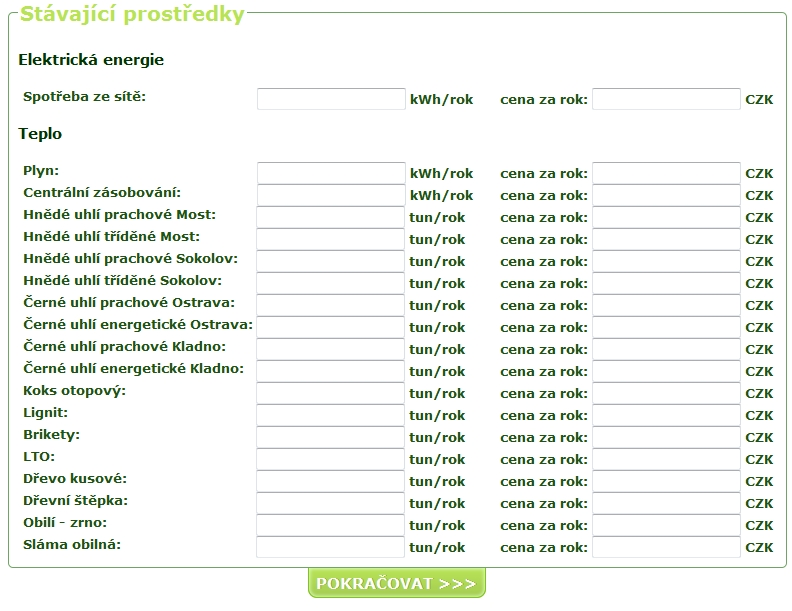
\includegraphics[scale=0.6]{DTOZE_formular_navrhB} 
\label{fig:formular_navrhB}
\end{figure} 

\begin{figure}[H] 
\centering 
\caption{Návrh formuláře DTOZE část dostupné kapacity} 
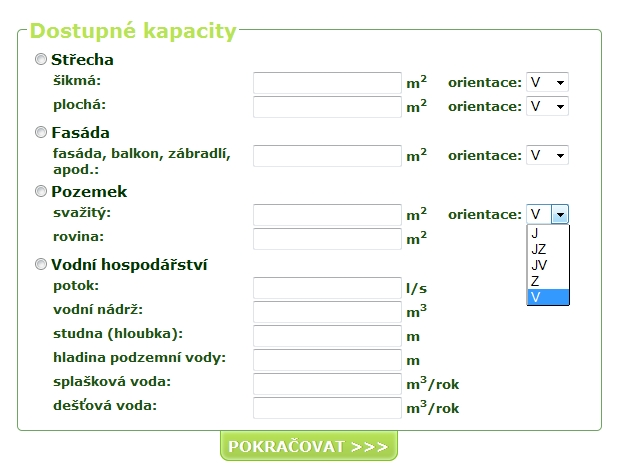
\includegraphics[scale=0.6]{DTOZE_formular_navrhC} 
\label{fig:formular_navrhC}
\end{figure} 

\subsubsection{Nalezení vhodného řešení} 
Vstupní data jsou využita především pro určení produktu, který je pro uživatele dostupný ať už z~finanční stránky, či z hlediska umístění. Každá technologie je svázána s umístěním. Např. FTV panel lze umístit na střechu rodinného domu či bytu nebo na fasádu či pozemek. Naopak studnu či vodní nádrž lze využít při výrobě elektrické energie tepelným čerpadlem. Dle umístění se odvíjí i parametr pro přepočet výkonu. Např. u fotovoltaiky je důležité, jak budou panely orientovány. Při orientaci na jih mají největší výkon, na západ či východ je např. výkon menší. Parametr pro přepočet výkonu je důležitý až ve výpočtech, na hledání vhodného řešení nemá vliv. Přehled předpokládaných technologií, které budou dostupné v databázi, jejich umístění a další specifikace jsou znázorněny v tabulce č. \ref{fig:umisteni_technologii}.

\begin{table}[H] 
\centering 
\caption{Umístění a další specifikace technologií v DTOZE} 
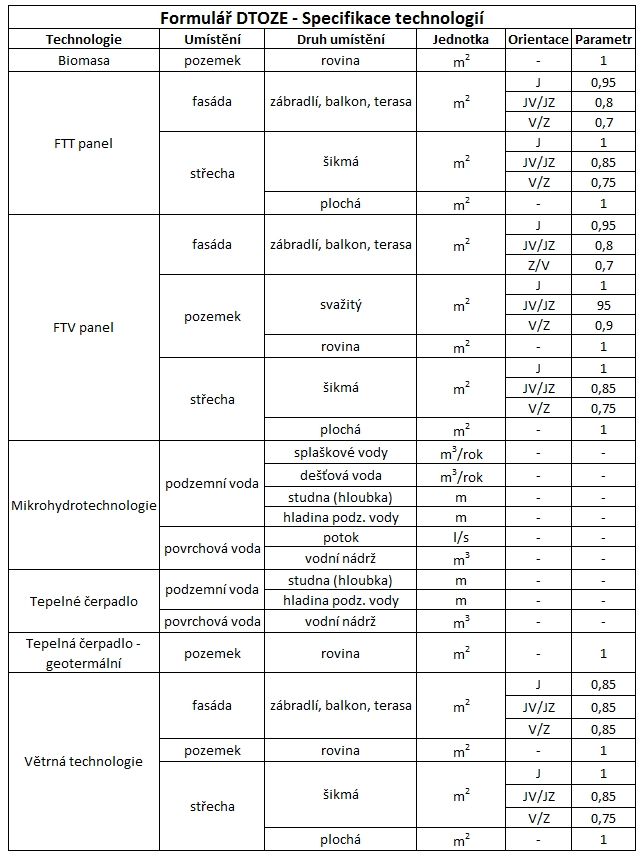
\includegraphics[scale=0.54]{Formular_DTOZE_spectechnol} 
\label{fig:umisteni_technologii}
\end{table} 

Od uživatele je získána informace o dostupných prostředcích v českých korunách (CZK) a informaci o dostupných kapacitách. Jedná-li se o plochu, je získána informace i o rozměru, u vodního hospodářství i o průtoku či výšce hladiny. Tyto informace stačí pro vyhledání vhodného řešení. Cílem je najít takové produkty, které vyhovují zadanému umístění a dostupným prostředkům. Dotaz do databáze v~zjednodušeném jazyce vypadá následovně: 

\noindent \textit{Najdi všechny technologie, které lze umístit na zadané umístění. Dále najdi všechny produkty, které vyhovují nalezeným technologiím. Podle zadaných dostupných prostředků odstraň z množiny výsledků produkty u kterých je údaj cena vyšší, než je zadáno, a které nesplňují podmínku umístění (např. je-li uveden rozměr, zkontroluj zda se daný produkt vejde do rozměru zadaného uživatelem, je-li uveden minimální průtok, zkontroluj zda je splněn). Takové produkty seřaď podle ceny a zobraz jejich název, technologii, fotku pokud je dostupná a cenu pokud je dostupná.}

Uživatel smí zadat pouze jedno umístění. V případě změny se může vrátit pouze k formuláři dostupné kapacity a vyplnit umístění znovu bez vyplňovaní předchozích formulářů. V případě, že bude produkt splňovat technologii a cenu nebo doplňující údaje nebudou uvedeny, zařadí se na konec vyhledaných produktů s informací o této skutečnosti. Systém si dle umístění zjistí parametr $par$ pro přepočet výkonu, který je použit v dalších výpočtech. 

\subsubsection{Výpočet výhodnosti investice}
Stěžejním výpočtem je výpočet výhodnosti investice do konkrétního produktu. Hlavní pro tento výpočet je, aby měl produkt v databázi definované potřebné údaje. V případě, že tyto údaje budou chybět, nelze provést výpočet.

\subsubsubsection{Výpočet ceny za spotřebovanou kilowatthodinu}
Než lze přejít k samotnému výpočtu výhodnosti konkrétní investice je nutné provést výpočet ceny za spotřebovanou kilowatthodinu (kWh). Výsledkem je cena elektrické energie, za kterou uživatel zaplatil/zaplatí (předpokládá se, že stáří údajů bude maximálně jeden rok.). Ta se vypočítá z informací získaných z formuláře v oddílu stávající infrastruktura. Konkrétně se jedná o odběr elektrické energie ze sítě, získávání tepla a cena za rok využívání. Výsledkem je cena za kWh. Výpočet se řídí dle vzorce (1), kde $p$ je cena za jednotku (CZK/kWh),  $P_{t}$ je cena spotřebovaného paliva za rok (CZK) a $C_{t}$ je spotřeba elektrické energie za rok (kWh): 

\begin{equation}
p = P_{t} / C_{t}
\end{equation}

\noindent V případě elektrické energie ze sítě je údaj rovnou v kWh, v případě tepla je nutné přepočíst počet tun na kWh. K dispozici jsou konstanty pro přepočet tun na kWh pro uvedené druhy paliv, které znázorňuje tabulka č. \ref{fig:vyhrevnost}.

\begin{table}[H] 
\centering 
\caption{Výhřevnost paliv na 1 tunu materiálu (zdroj: interní materiály firmy ECO trend)} 
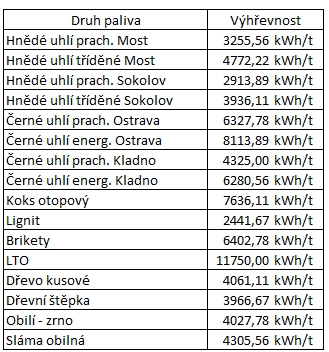
\includegraphics[scale=0.6]{Formular_DTOZE_vyhrevnost} 
\label{fig:vyhrevnost}
\end{table} 

Cena za jednotku z údajů o teple je ale ještě ovlivněna v případě, že je vyplněno více druhů paliv. V~tomto případě se vychází z průměrné ceny za jednotku ze všech paliv. Výpočet se tedy řídí dle vzorce (2), kde $p$ je cena za jednotku (CZK/kWh), $n$ je počet paliv, $P_{t}$ je cena spotřebovaného paliva za rok (CZK), $W_{t}$ je váha spotřebovaného paliva za rok (v tunách) a $k$ je konstanta výhřevnosti (kWh/t): 

\begin{equation}
p = \frac{\sum_{i=0}^{n} {\frac{P_{it}}{W_{it} * k}}}{n}
\end{equation}

V případě vyplnění údajů o elektrické energii i tepla zároveň se cena ještě jednou zprůměruje. 
\vspace{0.5cm}

\subsubsubsection{Výpočet efektivnosti investice}
Pro výpočet efektivnosti investice existuje několik postupů. Důležité ale je, aby dodržovaly určité zásady:\footnote{KNÁPEK, Jaroslav, Oldřich STARÝ a Jiří VAŠÍČEK. Zásady hodnocení ekonomické efektivnosti energetických projektů. \textit{Metodika EFEKT} [online]. 2003 [cit. 2014-04-12]. Dostupné z: \url{http://efekt.xf.cz/metodikaEFEKT.pdf}. Str.~2.}

\begin{itemize}
\item výpočet je založen na Cash Flow (peněžný tok, dále jen CF);
\item ve výpočtu jsou zahrnuty správné položky (např cena peněz v čase, diskont).
\item výpočet počítá s v nominálních cenách, respektuje cenový vývoj jednotlivých položek příjmů a~výdajů;
\item ve výpočtu je vhodně zvolena doba hodnocení a zahrnuje případné důsledky projektu po skončení zvolené doby;
\item počítá se s ohledem na důsledky financování.
\end{itemize}  

Problémem může při počítání efektivnosti investice být, že se měří penězi. U ekologicko-energetických projektů hraje roli mnoho faktorů, které nelze vyčíslit penězi. Příkladem může být ochránění přírodního prostředí, zlepšení zdraví apod. Výpočtem efektivnosti investice lze získat informace o tom, kolik to bude stát a jaký bude mít investice ekonomický efekt, avšak do rozhodování je nutné zvážit i další neměřitelné faktory, které mají pro investora význam.\footnote{Tamtéž str.~2-3.}

Ze zásad uvedených výše je patrné, že je důležité stanovit dobu hodnocení a vypočítat CF za daný rok se všemi položkami, které je nutné zahrnout. Doba hodnocení bude stanovena dle životnosti daného produktu. CF je nutné složit z položek: přímá úspora $S_{t}$ (která bude uspořena např. při neplacení elektrické energie ze sítě, či paliva za daný rok - výpočet z údajů, které zadal uživatel a z údajů v~databázi) a provozní náklady $C_{t}$ (nákup paliva, energie, instalace, údržba pozemku, apod., - výpočet z~údajů, které zadal uživatel a z údajů v~databázi). Vzorec (3) uvádí výpočet přímé úspory, která se vypočítá z roční výtěžnosti $Y_{t}$ a ceny za jednotku, která je získána z předchozího výpočtu. U některých technologií se stářím ubývá výkon, což je nutné zavést do výpočtu. $Y_{bt}$ je pak výkon v předchozím roce a $LP$ je zmiňovaný úbytek výkonu.\footnote{Tamtéž str.~4.} Některé technologie mají různý výkon dle orientace umístění, je tedy nutné výkon ještě vynásobit hodnotou parametru $par$, kterou si systém pamatuje od vyplnění formuláře o dostupných kapacitách. 

\begin{equation}
 S_{t} = p * ((Y_{bt} - LP ) * par) 
\end{equation}

Dále je potřeba vyčíslit provozní náklady. Ty se stanoví dle údajů od uživatele (např. u pozemku zadá, kolik ho přibližně stojí údržba za rok). Dále každý produkt může mít ještě další individuální provozní náklady (např. cena instalace, údržba, apod.). Provozní náklady získané od uživatele jsou značeny $C_{ut}$ a $C_{pt}$ jsou provozní náklady konkrétního produktu. Celkové provozní náklady se získají prostým součtem, jak znázorňuje vzorec (4).

\begin{equation}
C_{t} = (C_{ut} + C_{pt})
\end{equation}

Nyní jsou k dispozici veškeré údaje k vypočtení CF za daný rok. Vzorec (5) uvádí tento výpočet, za předpokladu, že investor využívá produkt pro vlastní potřebu, veškerou energii spotřebuje (nepřeprodává) a nevyužije investiční úvěr.

\begin{equation}
CF_{t} =  S_{t} - C_{t}
\end{equation}

Správné kritérium by mělo být založeno na maximalizaci budoucích CF. Takovým výpočtem je čistá současná hodnota ($NPV$ - Net Present Value), která převádí CF na sčitatelnou hodnotu s ohledem na cenu peněz v čase diskontováním od zvoleného okamžiku (např. od počátku provozu). Vzorec (6) počítá s $CF$ v daném roce, vloženou investicí $IN$ a s diskontní sazbou $r$, kde $Tv$ je doba životnosti a~$t$~je hodnocené období.\footnote{KNÁPEK, Jaroslav, Oldřich STARÝ a Jiří VAŠÍČEK. Zásady hodnocení ekonomické efektivnosti energetických projektů. \textit{Metodika EFEKT} [online]. 2003 [cit. 2014-04-12]. Dostupné z: \url{http://efekt.xf.cz/metodikaEFEKT.pdf}. Str.~5.}

\begin{equation}
NPV = \sum_{t=1}^{Tv} CF_{t} * (1+r)^{-t} - IN
\end{equation}

Důležité je stanovit správný diskont, neboli procento o které je budoucí výnos každoročně snížen při přepočtu na současnou hodnotu. Tato hodnota by měla být srovnatelná s možným výnosem alternativní investice. Používá se obvykle diskont s tzv. rizikovou přirážkou, tedy úroková sazba státních dluhopisů s dobou splatnosti srovnatelnou s dobou návratnosti uvažované investice a přirážka (kolem 2\%). V~případě drobných investorů (např. domácnosti) lze počítat s přiměřeným diskontem 3 \% (alternativní investicí může být např. dlouhodobý termínovaný vklad a i riziková přirážka může být menší).\footnote{BECHNÍK, Bronislav. Fotovoltaika jako náhrada biopaliv v dopravě.  \textit{tzbinfo.cz: stavebnictví, úspory energií, technická zařízení budov} [online]. 2. 9. 2013 [cit. 2014-04-12]. Dostupné z: \url{http://oze.tzb-info.cz/fotovoltaika/10291-fotovoltaika-jako-nahrada-biopaliv-v-doprave}.} Při možnosti využití pozemku se ještě připočítá rentabilita tohoto pozemku (např. má-li investor pole v~úrodné oblasti, rentabilita bude vyšší než v~neúrodné). Tuto hodnotu musí zadat uživatel, jinak s ní nebude počítáno. Vzorec pro NPV je vzorcem (7), kde $r_{pu}$ je rentabilita pozemku zadaná uživatelem v~procentech.
 
\begin{equation}
NPV = \sum_{t=1}^{Tv} CF_{t} * (1 + (r + r_{pu})^{-t} - IN
\end{equation}

Hodnota, která vyjde zahrnuje tři případy. Pokud je $NPV$ záporné, není vhodné do projektu investovat, v případě že je $NPV$ kladné lze investici doporučit, neboť výnos z projektu je vyšší než vložené investice. Posledním případem je, že je $NPV$ rovno nule, což značí, že výnos z projektu je stejný jako vložená investice. U investic do technologií využívajících OZE může být tento případ, nebo i mírně záporné $NPV$ kladným výsledkem, jelikož je nutné zohlednit zmiňované nezpeněžitelné důsledky na životní prostředí. V případě, že se posuzuje více investic zároveň, vybírá se taková, která má největší $NPV$. 

Výhodou kritéria je, že splňuje výše specifikované zásady správného hodnocení investic. Nevýhodou naopak je, že se musí správně stanovit doba životnosti a diskontní sazba. 

Dalším kritériem, které lze využít pro hodnocení investic je vnitřní výnosové procento ($IRR$ - Internal Rate of Return). Tato hodnota uvádí, jaká diskontní sazba dává právě nulovou hodnotu diskontovaného CF v dané době životnosti. Zjednoduše lze uvést, že $IRR$ je právě taková diskontní sazba $r$, kdy $NPV = 0$. Vzorec pro vypočtení $IRR$ je vzorcem (8).\footnote{KNÁPEK, Jaroslav, Oldřich STARÝ a Jiří VAŠÍČEK. Zásady hodnocení ekonomické efektivnosti energetických projektů. \textit{Metodika EFEKT} [online]. 2003 [cit. 2014-04-12]. Dostupné z: \url{http://efekt.xf.cz/metodikaEFEKT.pdf}. Str.~5-6.}

\begin{equation}
\sum_{t=1}^{Tv} CF_{t} * (1 + IRR)^{-t} - IN = 0
\end{equation}

Pro vyhodnocení zda se vyplatí investovat je opět nutné znát diskontní sazbu. V případě, že je $IRR$ větší nebo rovno než $r$, je vhodné investici realizovat, v opačném případě ne. Opět platí pravidlo, že je výhodnější investice s větším $IRR$.

Toto kritérium též splňuje zmiňované zásady, má však mnohem více nevýhod. Z matematického hlediska to není jednoznačný výpočet, může dojít k situaci, že reálná hodnota $IRR$ neexistuje. Dále nelze použít ve výpočtu různý diskont v různých letech, což $NPV$ dovoluje.\footnote{Hodnocení investic: Vnitřní výnosové procento (IRR).  \textit{BussinesVize.cz} [online]. 9. 11. 2010 [cit. 2014-04-12]. Dostupné z: \url{http://www.businessvize.cz/rizeni-a-optimalizace/hodnoceni-investic-vnitrni-vynosove-procento-irr}.}

Často používané kritérium při rozhodování je doba návratnosti. Prostá doba návratnosti ($PP$ - Payback Period) udává v jakém časovém horizontu převýší součet CF výši investice, dle vzorce (9).

\begin{equation}
\sum_{t=1}^{PP} CF_{t} - IN \excleq 0
\end{equation}

Kritériem je získat menší PP než je doba životnosti. Toto kritérium ale neuvažuje cenu peněz v čase a CF po ušlé době. Není proto vhodné se dle tohoto kritéria řídit, může být ale použito jako rychlý orientační údaj.\footnote{KNÁPEK, Jaroslav, Oldřich STARÝ a Jiří VAŠÍČEK. Zásady hodnocení ekonomické efektivnosti energetických projektů. \textit{Metodika EFEKT} [online]. 2003 [cit. 2014-04-12]. Dostupné z: \url{http://efekt.xf.cz/metodikaEFEKT.pdf}. Str.~6.}

Vylepšeným výpočtem je diskontovaní doba návratnosti (DPP - Discounted Payback Period). Vypočítá se pomocí již zmiňované diskontní sazby $r$ podle CF v jednotlivých rocích hodnocení dle vzorce~(10).

\begin{equation}
\sum_{t=1}^{DPP} CF_{t} * (1 - r)^{-t} - IN \excleq 0
\end{equation}

Pro tento výpočet platí stejné kritérium jako pro prostou dobu návratnosti, tedy minimalizovat $DPP$. Tento výpočet již respektuje cenu peněz v čase, avšak stále zanedbává CF po uplynutí $DPP$. Proto není vhodné hodnotit investici pouze na základě tohoto kriteria. 

V rámci aplikace využiji všechny zmiňované pohledy na hodnocení investice. Uživatel bude mít tedy možnost posoudit hodnoty všech zmiňovaných kritérií. V rámci aplikace bude u každé hodnoty krátká informace, co daný výsledek udává a zda investici doporučit či nikoli. Uživatel bude upozorněn, že tato doporučení jsou pouze orientační a nemusí plně odpovídat skutečnosti. 

\newpage
\section{Návrh databáze}
Návrh databáze je velmi důležitý pro budoucí implementaci. Vytváří můstek mezi požadavky a implementací. Snaží se zachytit vztahy, které mohou nastat, aby bylo zaručeno, že jsou všechny požadavky správně pochopeny a budou správně naimplementovány.\footnote{CONOLLY, Thomas, Carolyn BEGG a Richard HOLOWCZAK. \textit{Mistrovství - databáze: profesionální průvodce tvorbou efektivních databází.} Vyd. 1. Brno: Computer Press, 2009, 584 s. ISBN 978-80-251-2328-7. Str. 207.}

Definice metodiky z~knihy Mistrovství – databáze zní: „Proces vytvoření návrhu, který bude podporovat celkové poslání a dílčí cíle pro požadovaný databázový systém organizace.“\footnote{Tamtéž str. 206.}

Návrh databáze je jedna z~fází životního cyklu vývoje databázového systému. Předchází jí fáze plánování databáze, definice systému, sběr a analýza požadavků, které jsem popsala v předchozích kapitolách, a po ní následuje implementace databáze, testování a provozní údržba. 

Proces návrhu databáze se skládá z dalších tří fází – konceptuální návrh, logický návrh a fyzický návrh. Během konceptuálního návrhu se identifikují objekty, které je v~databázi nutné uchovávat, a~vztahy mezi nimi. V~logickém návrhu se identifikované objekty i vztahy přetváří na množinu tabulek. V~poslední fázi se rozhoduje, jak je nutné tabulky fyzicky implementovat.\footnote{Tamtéž str. 207.} Podrobněji o~jednotlivých fázích pojednávají následující kapitoly. Při tvorbě návrhu se řídím dle metodologie popsané v~knize Mistrovství – databáze.\footnote{CONOLLY, Thomas, Carolyn BEGG a Richard HOLOWCZAK. \textit{Mistrovství - databáze: profesionální průvodce tvorbou efektivních databází.} Vyd. 1. Brno: Computer Press, 2009, 584 s. ISBN 978-80-251-2328-7.} Jednotlivé kroky doplňuji tvorbou samotné databáze, dle požadavků zadavatele. 

Návrh databáze níže popsaný je určen pro návrh relační databáze. Pro vizualizaci návrhu používám nástroj Enterprise Architect a objektově orientovaný jazyk UML (Unified Modeling Language). 

\subsection{Konceptuální návrh}
V~této fázi návrhu se vytváří konceptuální model dat neboli ER (entity relation) model. Vychází z~informací, které byly ujednány v~rámci požadavků, z~nichž identifikuje důležité entity a relace, které je nutné zachytit v~požadované databázi. V~rámci tvorby modelu se dbá mimo jiné i na minimalizování redundancí. V~následujících kapitolách popisuji postup při vytváření konceptuálního modelu. 

\subsubsection{Identifikace entit}
Nejdříve je nutné ujasnit, jaké entity bude v~databázi potřeba ukládat. Projdou se nasbírané informace od zadavatele databáze a vytvoří se slovník dat, kde je uveden název entity, popis a předpokládaný počet výskytů. K těmto entitám je důležité zahrnout i další entity, které nebyly přímo zmíněny, ale bude je nutné na základě fungování systému uvážit. Všechny entity by měly mít velmi podrobný popis a informace o datech, které budou obsahovat. Již nyní je tedy důležité mít hrubou představu o tom, jak bude systém pracovat. Obsah slovníku není neměnný a v průběhu návrhu se může ještě změnit. Slovník pro DTOZE znázorňuje tabulka č. \ref{fig:navrh_slovnik}.

\begin{table}[H] 
\centering 
\caption{Slovník DTOZE z předpokládaným počtem entit za rok existence} 
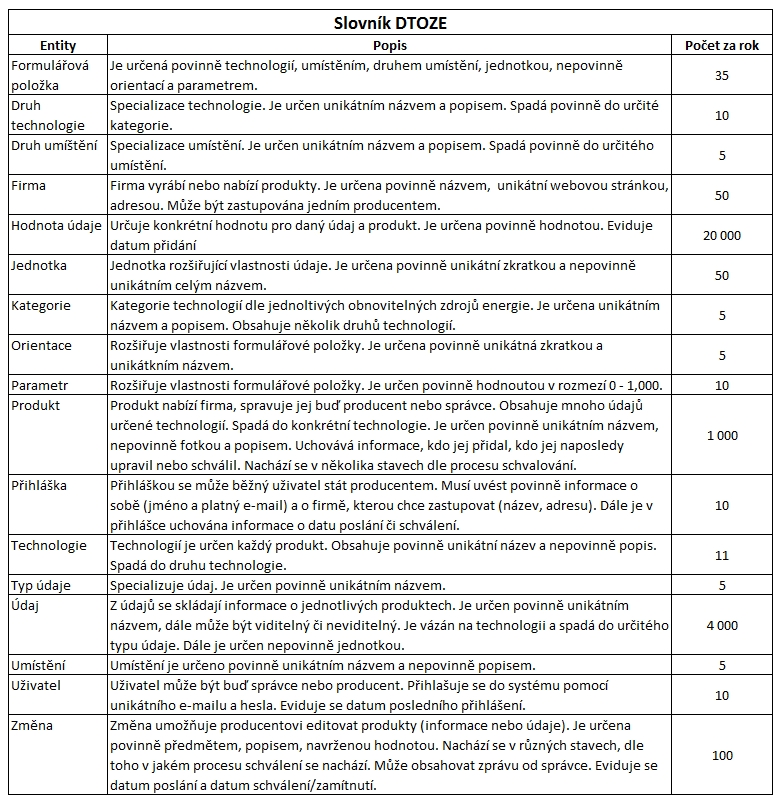
\includegraphics[scale=0.57]{DTOZE_konc_slovnik} 
\label{fig:navrh_slovnik}
\end{table} 

\subsubsection{Identifikování relací}
Dalším krokem je identifikace relací (vztahů) mezi jednotlivými entitami. Pro definování vztahu se vychází ze slovníku, či je nutné se opět vrátit k~požadavkům na databázi. Typicky se relace označují slovesy.  

Vztah je definován zpravidla mezi dvěma entitami. Vztahem může vzniknout i vazební entita, která obsahuje informace společné pro obě entity ve vztahu. Lze definovat vztah nad jednou entitou. Pak se takový vztah nazývá samoreferenční nebo také rekurzivní. Vzniknout může i n-ární vztah, tedy ve~vztahu jsou více než dvě entity, ale tento typ vztahu je výjimečný.\footnote{HERNANDEZ, Michael J. a HOLOWCZAK. Návrh databází. 1. vydání. Praha: Grada, 2006, 408 s. Profesional. ISBN 80-247-0900-7. Str. 227-232.}

Speciálním vztahem je dědičnost - tedy vztah nadtřída/podtřída. Nadtřída je entita, která obsahuje obecné atributy, společné pro více entit. Tyto entity se nazývají podtřídy a dědí atributy nadtřídy. Nadtřídy i podtřídy je nutné v~diagramu samostatně reprezentovat. Vztah mezi nadtřídou a kteroukoli její podtřídou je 1:1 a značí se plnou šipkou bez viditelných multiplicit. Každá podtřída je členem nadtřídy, ale s~konkrétnější rolí.\footnote{CONOLLY, Thomas, Carolyn BEGG a Richard HOLOWCZAK. \textit{Mistrovství - databáze: profesionální průvodce tvorbou efektivních databází.} Vyd. 1. Brno: Computer Press, 2009, 584 s. ISBN 978-80-251-2328-7. Str. 178-179.} 

Např. v~návrhu DTOZE existuje entita uživatel, která má dvě role - producent a správce. Uživatelé mají mnoho společných vlastností (jméno, e-mail, heslo, atd.) a několik specifických pro danou roli (správce může upravovat všechny produkty, správce pouze ty, které přidal, atd.). V tomto případě se neliší v atributech, pouze ve vztazích a proto není nutné dědičnost zavádět. V případě, že by producent musel uvést telefon a správce by měl navíc vazby na práva k přístupu k úpravě dat, bylo by vhodné tuto skutečnost implementovat skrze dědičnost. Ukázka implementace dědičnosti je znázorněna na obrázku č.~\ref{fig:dedicnost}.

\begin{figure}[H] 
\centering 
\caption{Ukázka vztahu dědičnosti} 
\vspace{0.2cm}
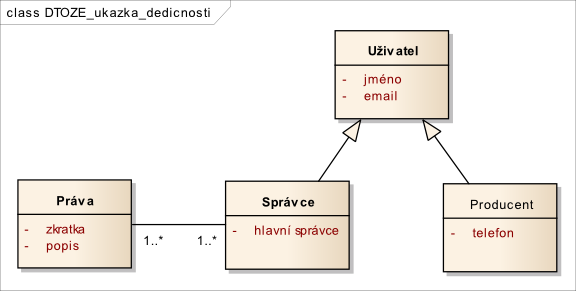
\includegraphics[scale=0.6]{dedicnost_n} 
\label{fig:dedicnost}
\end{figure} 

V případě zachycení pouze jednou entitou, by se do tabulky zanášely hodnoty NULL\footnote{NULL je nedefinovaná hodnota, která ale není číselná ani textová. Hodnota je to neznámá či neplatná pro daný záznam. CONOLLY, Thomas, Carolyn BEGG a Richard HOLOWCZAK. Mistrovství - databáze: profesionální průvodce tvorbou efektivních databází. Vyd. 1. Brno: Computer Press, 2009, 584 s. ISBN 978-80-251-2328-7. Str. 68.} ke sloupcům, které správce nebo producent nevyužije. To je jedním z~hlavních důvodů, proč se dědičnost zavádí. Druhým důležitým důvodem je zpřehlednění diagramu, kdy je zřejmé, s~čím je daná entita ve vztahu. V~případě, že by vše bylo v~jedné tabulce Uživatel, měla by tato entita vztah se vším a nebylo by jasně dané, která role je ve vztahu s~čím. 

Součástí relací je omezení multiplicity, která vymezují typy vztahů mezi relacemi. Těmito typy jsou vztahy 1:1 (každý záznam první entity je vázán právě s~jedním záznamem druhé entity), 1:N (jeden záznam první entity má jeden nebo více záznamů druhé entity) a N:M (jeden záznam první entity může mít několik záznamů druhé entity a zároveň druhý záznam entity může mít několik záznamů první entity). Multiplicity pak mohou být specifikovány několika typy, dle toho zda je multiplicita nepovinná (0..1, 0..*) či povinná (1..1,1..*).\footnote{HERNANDEZ, Michael J. a HOLOWCZAK. Návrh databází. 1. vydání. Praha: Grada, 2006, 408 s. Profesional. ISBN 80-247-0900-7. Str. 227-232.}

Relace se nejdříve zanesou do tabulky a následně je vhodné je znázornit v~diagramu. Vztahy entit DTOZE jsou vypsány v~tabulce~č. \ref{fig:DTOZE_konc_vztahy} a na obrázku~č. \ref{fig:DTOZE_konc_bezA} jsou znázorněny v~diagramu.

\begin{table}[H] 
\centering 
\caption{Vztahy mezi entitami DTOZE} 
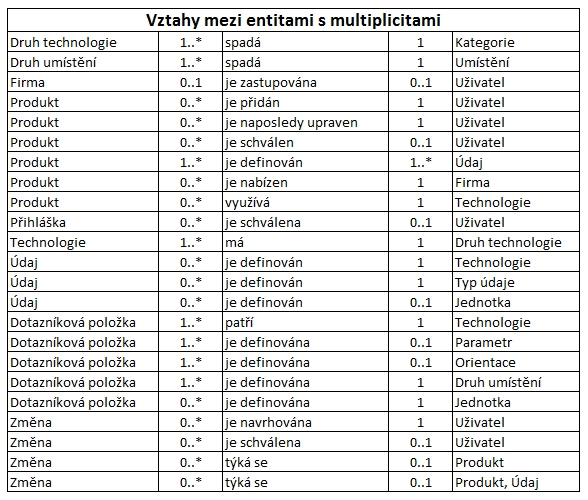
\includegraphics[scale=0.55]{DTOZE_konc_vztahy}
\label{fig:DTOZE_konc_vztahy} 
\end{table} 

\begin{figure}[H] 
\centering 
\caption{ER diagram DTOZE} 
\vspace{0.1cm}
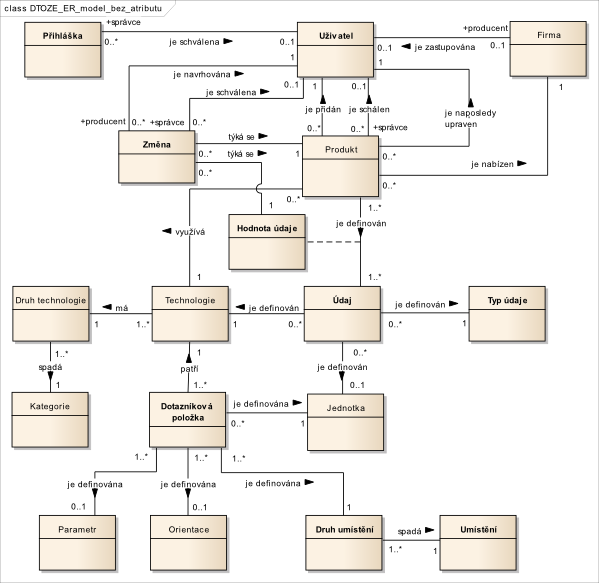
\includegraphics[scale=0.75]{DTOZE_konc_bezA_n} 
\label{fig:DTOZE_konc_bezA}
\end{figure} 
\newpage

\subsubsection{Určení atributů a primárních klíčů}
Žádná entita nemá význam bez dalších informací. Tyto informace se shromažďují pomocí atributů. K~určení atributů je nutné opět prozkoumat slovník dat. Atributy jsou např. vlastnosti, jakost, charakteristika apod. Dělí se na jednoduché (odkazuje pouze na jednu hodnotu), složené (odkazuje na několik hodnot), odvozené (jejich hodnota je určena pomocí jiných atributů) a atributy relací (váže se k~relaci, nikoli pouze k~entitě).\footnote{CONOLLY, Thomas, Carolyn BEGG a Richard HOLOWCZAK. \textit{Mistrovství - databáze: profesionální průvodce tvorbou efektivních databází.} Vyd. 1. Brno: Computer Press, 2009, 584 s. ISBN 978-80-251-2328-7. Str. 214–216.}  

Mezi zvolenými atributy se vybírají kandidáti na primární klíč, který jednoznačně identifikuje každý záznam dané entity. Může to být jeden atribut, ale i složený. Takový kandidát nesmí nabývat NULL hodnoty. Z~kandidátů se pak vybírá jeden primární klíč na základě následujících kritérií: kandidát s~minimální množinou atributů; kandidát, u~něhož je nejméně pravděpodobná změna hodnot; kandidát s~nejmenším počtem znaků; kandidát s~nejmenší maximální hodnotou. Pokud neexistuje mezi existujícími atributy vhodný kandidát na primární klíč, je nutné vytvořit umělý primární klíč, např. číselný atribut ID (od slova IDentification).\footnote{Tamtéž str. 219.} 

Na obrázku~č. \ref{fig:DTOZE_konc_sA} je zobrazen ER diagram již s~atributy a určenými primárními klíči. Při určování primárních klíčů se mi nepodařilo najít vhodného kandidáta, a proto je u~všech entit určen umělý klíč. Uvažovaným kandidátem byl u~některých entit název, ale u~něho nelze zaručit, že bude jednoduchý a neproměnlivý. Dále byl kandidátem na primární klíč např. atribut hodnota entity Parametr. Ten je sice unikátní a krátký, jelikož se jedná o číslo, ale je vyjádřen číslem s desetinnou čárkou a též nelze zaručit, že nebude proměnlivý.  

V diagramu jsou navíc zaneseny poznámky o omezení, které vyplynuly z požadavků, avšak v rámci vztahů je nelze zanést do modelu. Tyto poznámky jsou důležité pro dále pro logický a fyzický návrh či pro samotnou implementaci.

\begin{figure}[H] 
\centering 
\caption{ER diagram s~atributy a vyznačenými primárními klíči (podtržené)} 
\vspace{0.1cm}
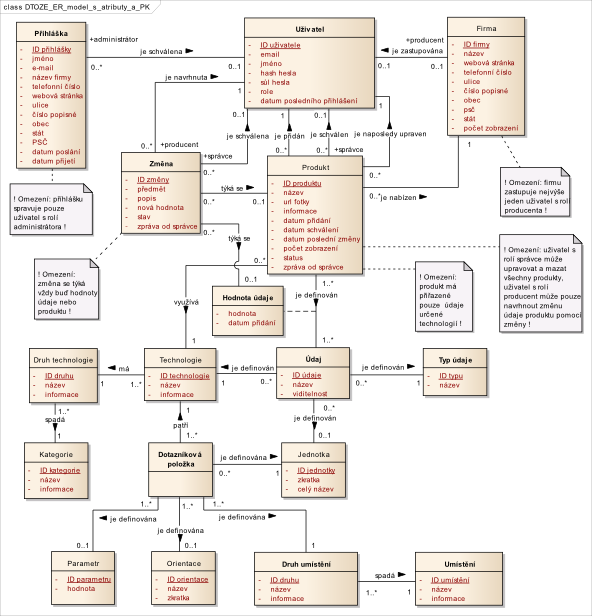
\includegraphics[scale=0.75]{DTOZE_konc_sA_n} 
\label{fig:DTOZE_konc_sA}
\end{figure} 

\subsubsection{Kontrola redundance}
Splněním předchozích kroků je model téměř hotový. Jelikož je model postupně rozšiřován, je možné, že do něj byly zanesly redundance - nadbytečně zaznamenané informace. Ty mohou být zaneseny buď v~entitách, nebo v~relacích. K~odstranění případných redundancí v~entitách je nutné zpětně prozkoumat vztahy 1:1 a atributy jednotlivých entit. Tam by se mohla omylem vyskytnout entita stejná jako jiná, pouze pojmenovaná synonymem. Relace je redundantní pokud vyjadřuje informaci, kterou lze získat prostřednictvím jiné relace. V~modelu se vyhledají entity, které mají několik relací a znovu se posuzuje význam a účel.\footnote{CONOLLY, Thomas, Carolyn BEGG a Richard HOLOWCZAK. \textit{Mistrovství - databáze: profesionální průvodce tvorbou efektivních databází.} Vyd. 1. Brno: Computer Press, 2009, 584 s. ISBN 978-80-251-2328-7. Str. 220–222.}

U mého návrhu se nevyskytují žádné vztahy 1:1 a problém jsem nalezla pouze u entity Přihláška, kde je mnoho dat zaneseno redundantně zároveň v entitách Uživatel a Firma. Tato redundance je ale záměr. Je nutné ukládat poslané přihlášky odděleně od zveřejněných dat, jelikož je pravděpodobné, že všechny přihlášky nebudou přijaty a zaneseny rovnou do databáze, jelikož nebudou splňovat podmínky pro přijetí.

\subsection{Logický návrh}
Jestliže je hotový ER model (nebo také ER diagram), lze začít pracovat na logickém návrhu. Cílem je vytvořit detailní popis tabulek na základě entit z~konceptuálního modelu. Dále se tabulky normalizují, aby se opět zamezilo redundanci, tentokrát na úrovni sloupců tabulek. U~logického návrhu se držím následujícího postupu.

\subsubsection{Struktura tabulek}
V~této fázi se připraví struktura tabulek, která již bude použita ve fyzické databázi. Každá entita ER modelu nyní vyjadřuje tabulku a její atributy vyjadřují sloupce tabulky. K~popsání struktury se používá jazyk DBDL (Database Definition Language), díky kterému lze strukturu tabulky vyjádřit textem. Pravidla jsou následující: nejdříve se uvede jméno tabulky a poté v~závorce názvy sloupců. Primární klíče jsou opět zobrazeny podtrženě. V~případě DTOZE je struktura vyznačena na obrázku č.~\ref{fig:DTOZE_log_A}. 

\begin{figure}[H] 
\centering 
\caption{Struktura DTOZE pomocí DBDL} 
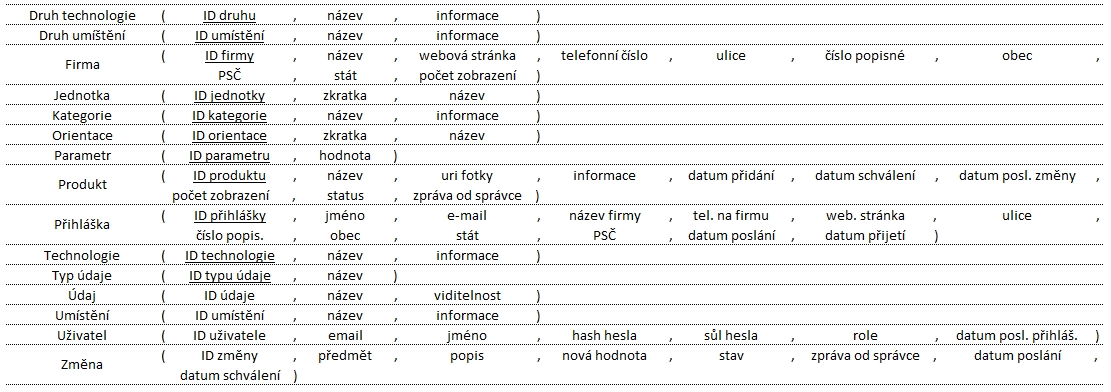
\includegraphics[scale=0.43]{DTOZE_log_A} 
\label{fig:DTOZE_log_A}
\end{figure} 

Při zaznamenávání relací přibudou k~tabulkám ještě další sloupce, a to cizí klíče.  Ty se identifikují na základě vztahu tabulek. Tabulky se podle vztahu rozlišují na rodičovské a dceřiné. Primární klíč rodičovské tabulky se přenáší jako cizí klíč (nový sloupec) do dceřiné tabulky. Je opět několik pravidel pro tvorbu cizích klíčů, kompletní shrnutí znázorňuje tabulka č.~\ref{fig:reprezentace_entit}\footnote{CONOLLY, Thomas, Carolyn BEGG a Richard HOLOWCZAK. \textit{Mistrovství - databáze: profesionální průvodce tvorbou efektivních databází}. Vyd. 1. Brno: Computer Press, 2009, 584 s. ISBN 978-80-251-2328-7. Str. 242.}. Aplikování na struktu DTOZE v~jazyce DBDL pak znázorňuje obrázek č.~\ref{fig:DTOZE_log_B}. Cizí klíče jsou zobrazeny tučně.

\begin{table}[H] 
\centering 
\caption{Shrnutí reprezentace entit, relací a atributů s~více hodnotami pomocí tabulek} 
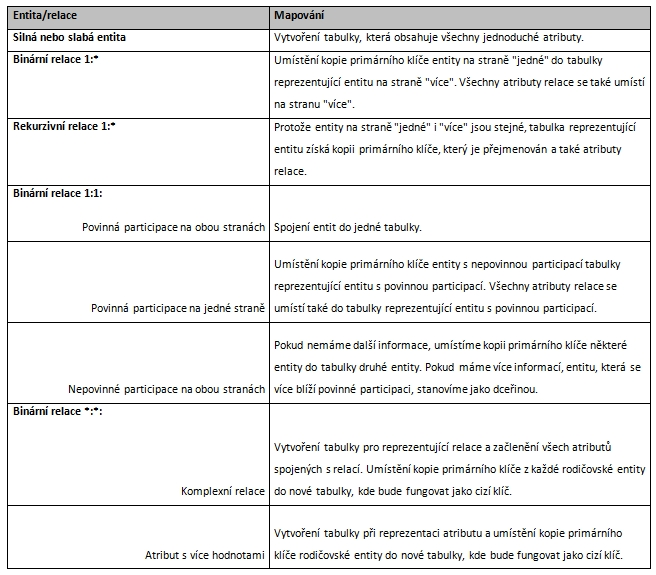
\includegraphics[scale=0.6]{vztahy} 
\label{fig:reprezentace_entit}
\end{table} 

\begin{figure}[H] 
\centering 
\caption{Struktura DTOZE pomocí DBDL po zavedení cizích klíčů} 
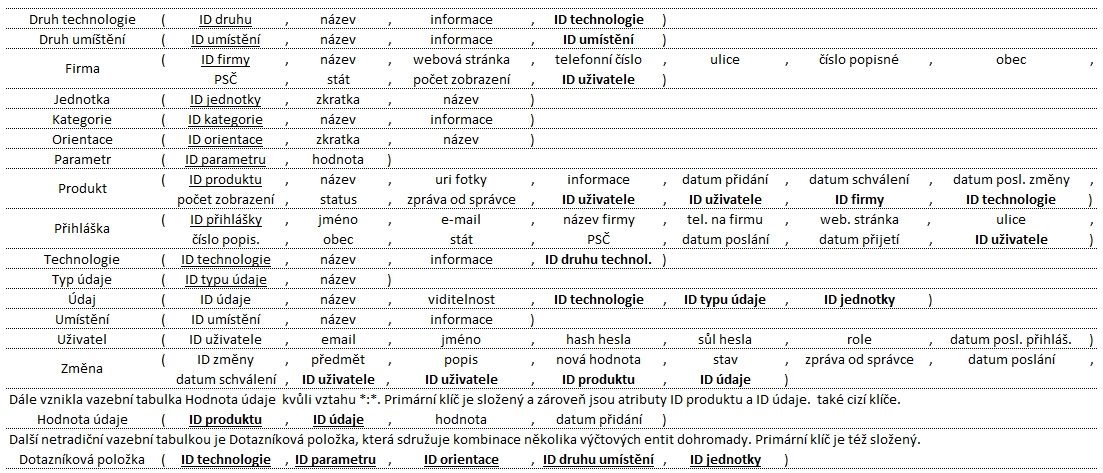
\includegraphics[scale=0.43]{DTOZE_log_B} 
\label{fig:DTOZE_log_B}
\end{figure} 
\newpage

\subsubsection{Kontrola tabulek pomocí normalizace}
Vytvořené tabulky a jejich relace je nyní nutné prověřit, zda neporušují některé z~normálních forem.  Normalizace je proces, při kterém se relace upravují za účelem jednodušší práce a lepší manipulace s~daty, zabránění redundance a lepší konzistence dat.  Definovány jsou tři základní normální formy: 1NF, 2NF, 3NF.\footnote{KULHAN, Jakub. Normalizace relačních databází. \textit{Programujte.com} [online]. 2008 [cit. 2013-12-10]. Dostupné z: \url{http://programujte.com/clanek/2008071900-normalizace-relacnich-databazi/}.} Čím vyšší normu logický návrh splňuje, tím se zpravidla lépe pracuje s~daty v~databázi.  

Tabulka je v~první normální formě (1NF), pokud neexistuje pole tabulky, které by obsahovalo více než jednu hodnotu. Např. pokud je v~tabulce uchována hodnota adresy v~jednom poli (tedy pole obsahuje ulici, číslo popisné, poštovní a směrovací číslo a město), pak taková tabulka není v~1NF. Řešením je vytvoření nové tabulky a vytvoření relace s~původní tabulkou. 

Aby byla tabulka v~druhé normální formě (2NF), musí všechna data záviset na celém klíči. V~případě, že bude nutné upravit pole, které není závislé na celém klíči, bude se muset změna zanášet na několik míst. To je ale nežádoucí. Řešením je rozložení původní tabulky na více tabulek, kde se závislost na necelém klíči vymění za cizí klíč. 

Třetí normální forma (3NF) udává, že všechny neklíčové atributy musí být navzájem nezávislé. Pokud by například byly v~tabulce atributy primární klíč ID osoby, jméno osoby, pobočka firmy, ve~které pracuje a adresa této pobočky, pak není tabulka ve 3NF, jelikož atribut adresa pobočky je závislá na atributu pobočky. Řešením je opět rozdělení na více tabulek. \footnote{SKŘIVAN, Jaromír. Databáze a jazyk SQL.  \textit{Interval.cz} [online]. 2000 [cit. 2013-12-10]. Dostupné z: \url{http://interval.cz/clanky/databaze-a-jazyk-sql/}.} 

Existují další normy: Boyce-Coddova normální forma (BCNF), čtvrtá normální forma 4NF a pátá normální forma (5NF).\footnote{CONOLLY, Thomas, Carolyn BEGG a Richard HOLOWCZAK. \textit{Mistrovství - databáze: profesionální průvodce tvorbou efektivních databází}. Vyd. 1. Brno: Computer Press, 2009, 584 s. ISBN 978-80-251-2328-7. Str. 199.} Tyto formy identifikují a řeší málo frekventované problémy, a proto je zde neuvádím.  

Dle postupů zmíněných výše je velice pravděpodobné, že se struktura tabulek po normalizaci může ještě změnit. Změny se zavedou do struktur tabulek a dále se s~nimi pracuje. Při vytváření struktur tabulek jsem již na normalizaci intuitivně myslela, a proto po přezkoumání tabulek DTOZE nedošlo ke změnám. Našla jsem však několik atributů, které by mohly potencionálně porušovat některou z~forem. Na obrázku č.~\ref{fig:DTOZE_log_C} je zobrazeno, v~jakých normách jsou tabulky DTOZE, a u~kterých je podezření na~porušení některých z~forem. Dále vysvětluji důvody, proč ke změnám tabulek nedošlo. 

\begin{figure}[H] 
\centering 
\caption{Normalizace tabulek DTOZE} 
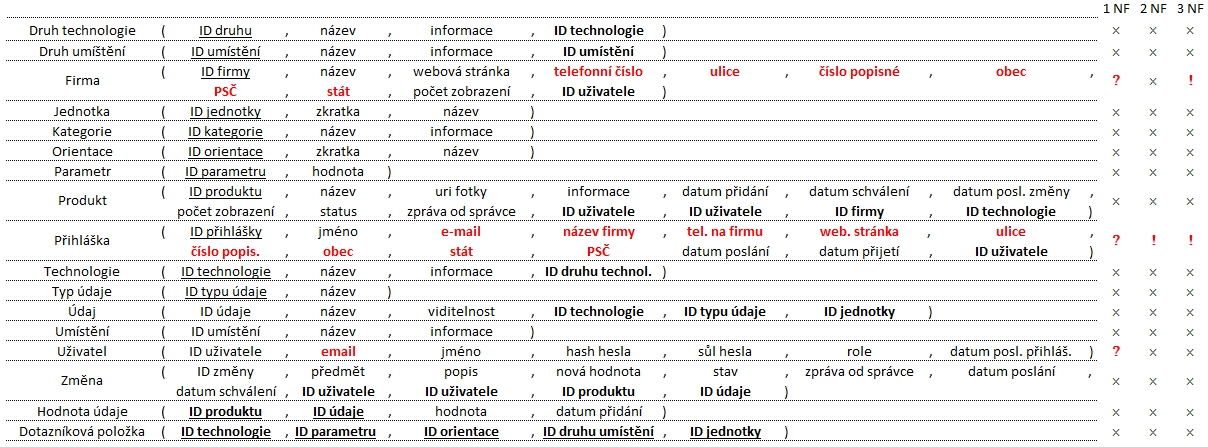
\includegraphics[scale=0.4]{DTOZE_log_C} 
\label{fig:DTOZE_log_C}
\end{figure} 

Dnes je již zcela běžné, že má člověk více telefonů či e-mailů. Mohlo by tedy dojít k~situaci, že uživatel při registraci nebude vědět, které údaje zadat. Řešením by bylo vytvořit další tabulky, které by umožňovaly konkrétnímu záznamu mít více zmíněných atributů. Uvážila jsem toto rozdělení za zbytečné, jelikož tyto kontakty mají sloužit uživatelům k~rychlému zorientování, kam se obrátit v~případě zájmu o~produkt. V~případě, že by bylo uvedeno více telefonních čísel či e-mailových adres, musel by uživatel řešit dilema na jaké se obrátit. V~databázi bude tedy povoleno mít pouze jeden kontaktní e-mail a jedno telefonní číslo u~entit, kterých se to týká. 

U~tabulky Přihlášky a Firmy se může zdát, že porušuje 2NF, jelikož obsahuje informace o~firmě, které jsou závislé na názvu firmy. Důležitý je zde fakt, že tabulka přihlášek slouží k~uchování všech dat zadaných uživatelem, který projevil zájem stát se producentem. Tato data by se již neměla po zapsání měnit, pouze se z~nich bude čerpat při přidávání záznamů do tabulek Producent, Firma. Tato tabulka není v~2NF (a tedy ani ve 3NF), ale struktuře naší databáze to nevadí. Dále ani entita Firma není v~2NF ani 3NF ze stejného důvodu. Firma obsahuje položky adresy. Ale na jedné adrese může být více firem, bude tedy docházet k redundancím. Navíc ulice, město a stát je určen PSČ, to by mělo být také v jiné tabulce. V tomto okamžiku je důležité, jak bude k těmto datům přistupováno a kolik firem bude v databázi zastoupeno. Předpokládá se, že firem v databázi mnoho nebude, ale přistupovat k detailům o firmách se bude relativně často. Proto je výhodnější opakovat některá data než je dohledávat v jiné tabulce.

Při normalizaci se dbá nejvíce na to, aby se data neopakovala a byla snadno upravitelná. V některých případech ale může být výhodnější jiné řešení. Tím se ale zabývám podrobněji až při fyzickém návrhu v kapitole č. \ref{cap:denormalizace} o denormalizaci. Při logickém návrhu není ještě důležité fungování databázového systému i když je už vhodné o efektivním uložení dat přemýšlet během celého navrhování databáze.
\newpage

\subsubsection{Kontrola integritních omezení}
Integritní omezení se zavádějí pro zaručení úplnosti, přesnosti a konzistence dat v~databázi. Jedná se~o:
\begin{itemize}
\item Požadovaná data – některé sloupce nesmí obsahovat hodnotu NULL.
\item Omezení množin přípustných hodnot – stanovení množiny hodnot, kterých může sloupec nabývat.
\item Multiplicita – přesně definovaná kardinalita (mohutnost) u~jednotlivých relací.
\item Referenční integrita – souvisí s~cizími klíči, pokud cizí klíč obsahuje hodnotu, pak tato hodnota musí odkazovat na existující záznam v~rodičovské tabulce.
\item Jiná integritní omezení – stanoví se na základě požadavků na databázi, platí pro konkrétní model.\footnote{CONOLLY, Thomas, Carolyn BEGG a Richard HOLOWCZAK. \textit{Mistrovství - databáze: profesionální průvodce tvorbou efektivních databází}. Vyd. 1. Brno: Computer Press, 2009, 584 s. ISBN 978-80-251-2328-7. Str. 247-250.}
\end{itemize}

Konkrétní nastavení těchto omezení už ale závisí na DBMS (database management system), který se použije pro implementaci. Je vhodné ale zvážit již předem, jak data omezit. Některá z~omezení, která lze nyní vyhodnotit jsou zaznamenaná v~logickém návrhu  v~tabulce č.~\ref{fig:DTOZE_log_D}. Jedná se o omezení NULL hodnot, unikátnosti sloupců, předpokládané množiny hodnot a velikosti. 

Dále byla vyhodnocena následující omezení, která se týkají více sloupců či tabulek nebo je nutné je vymezit speciálně. Na tato omezení je nutné brát ohled při fyzickém návrhu popř. při implementaci aplikace.

\begin{itemize}
\item Přihlášku může spravovat pouze jeden nebo žádný Uživatel s rolí správce.
\item Firmu může zastupovat pouze jeden nebo žádný Uživatel s rolí producenta.
\item Uživatel s rolí správce může upravovat a mazat všechny Produkty, Uživatel s rolí producent může pouze navrhnout editaci Údaje produktu pomocí Změny.
\item Změna se týká vždy buď Hodnoty údaje nebo Produktu.
\item Produkt má přiřazené pouze údaje určené technologií.
\item Datum přidání (poslání) musí být vždy stejné nebo starší než datum schválení. Datum schválení musí být vždy stejné nebo starší než datum poslední úpravy.
\item E-mail musí být v platném formátu.
\item URL adresy musí být v platném formátu.
\end{itemize}
\newpage

\begin{table}[H] 
\centering 
\caption{Logický návrh tabulek společně s~integritními omezeními.} 
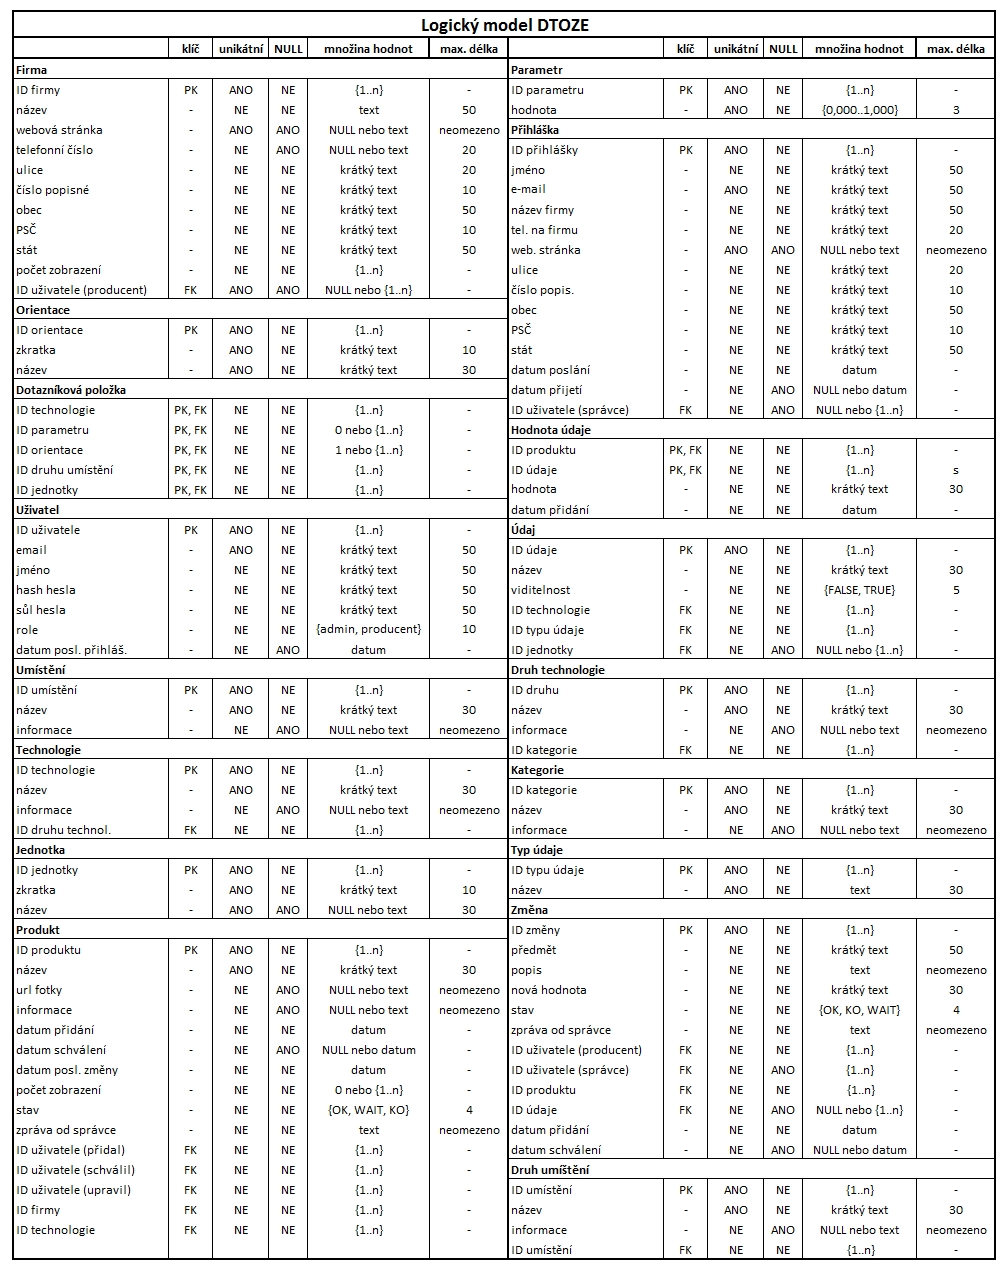
\includegraphics[scale=0.48]{DTOZE_log_D} 
\label{fig:DTOZE_log_D}
\end{table} 

\newpage

\subsection{Fyzický návrh}
Zatímco při logickém návrhu byla upřena pozornost na to, co bude obsahem databáze, při vytváření fyzického návrhu je hlavní otázka, jak to bude zprovozněno. Pro vytvoření fyzického návrhu je již nutné znát funkčnost cílového DBMS. 

DBMS je systém, který umožňuje komunikovat uživateli či aplikaci s databází. Existuje několik druhů DBMS - mezi nejznámější, založené na relačním ukládání, dat patří např. MySQL, Microsoft SQL Server, Oracle či PostgreSQL.\footnote{CONOLLY, Thomas, Carolyn BEGG a Richard HOLOWCZAK. \textit{Mistrovství - databáze: profesionální průvodce tvorbou efektivních databází}. Vyd. 1. Brno: Computer Press, 2009, 584 s. ISBN 978-80-251-2328-7. Str. 39.}

Komunikace je umožněna pomocí dotazovacího jazyka. U zmiňovaných relačních DBMS je to např. SQL (Structured Query Language). Jedná se o neprocedurální jazyk (nevyžaduje určení přístupové metody k datům), je relativně snadný pro naučení a pomocí něho lze přistupovat do databáze ať už kvůli konfiguraci databáze, či kvůli správě dat.\footnote{Tamtéž str. 76.} 

Každý databázový systém prošel různým vývojem a i když vychází ze stejného dotazovacího jazyka, může se od ostatních v některých ohledech lišit, např. v implementaci datových typů, programovacích strukturách či v některé syntaxi. Proto je pro fyzický návrh již důležité znát DBMS, v rámci kterého bude databáze implementována. Pro implementaci DTOZE jsem vybrala databázový systém PostgreSQL, jelikož je dostupný na zařízení, na kterém bude implementována celá aplikace. 

V rámci fyzického návrhu se vychází z logického návrhu. Zahrnuje návrh podkladových tabulek a~doplnění integritních omezení dle cílového DBMS, návrh a implementaci odvozených sloupců, analýzu transakcí, které mají být podporovány, zavedení indexů, implementování pohledů, zvážení denormalizace, návrh bezpečnostních opatření\footnote{Tamtéž str. 259.} a otestování vzniklé databáze.             

\subsubsection{Návrh tabulek a integritních omezení}
V tomto kroku se vychází z dat nashromážděných v rámci logického návrhu. Dochází zjednodušeně k~překladu tabulek z logického návrhu do jazyka SQL a syntaxe cílového DBMS a implementaci integritních omezení, popř. doplnění dalších.

Nejen pro vizualizaci lze opět využít některý z modelovacích nástrojů a vytvořit v něm databázový model. Databázový model nese mnohem více informací o jednotlivých tabulkách než ER model či logický model. Proto jsem model DTOZE rozdělila na tři logické celky, které budou čitelnější, než jeden veliký.

Databázový model DTOZE A, který je zobrazen na obrázku č.~\ref{fig:DTOZE_fyz_A} znázorňuje hlavní sturkturu databáze. Databázový model DTOZE B na obrázku č.~\ref{fig:DTOZE_fyz_B} rozšiřuje entity Uživatel (DTOZE\_User), Produkt(DTOZE\_Product), Hodnota údaje (DTOZE\_StatementValue) a Údaj (DTOZE\_Statement) o entitu Změna (DTOZE\_Change) a zachycuje v jakém jsou vztahu. Databázový model DTOZE C na~obrázku č.~\ref{fig:DTOZE_fyz_C} zobrazuje několikanásobný vztah Dotazníková položka (DTOZE\_SurveyItem) s~ostatními entitami, kterých se týká. 

\begin{figure}[H] 
\centering 
\caption{Databázový model DTOZE A} 
\vspace{0.1cm}
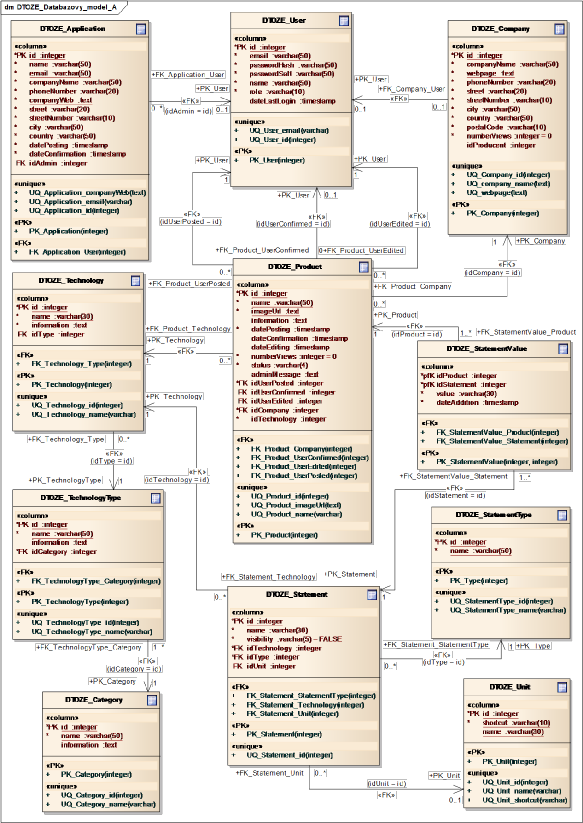
\includegraphics[scale=0.75]{DTOZE_fyzA_n} 
\label{fig:DTOZE_fyz_A}
\end{figure} 
\newpage

\begin{figure}[H] 
\centering 
\caption{Databázový model DTOZE B} 
\vspace{0.1cm}
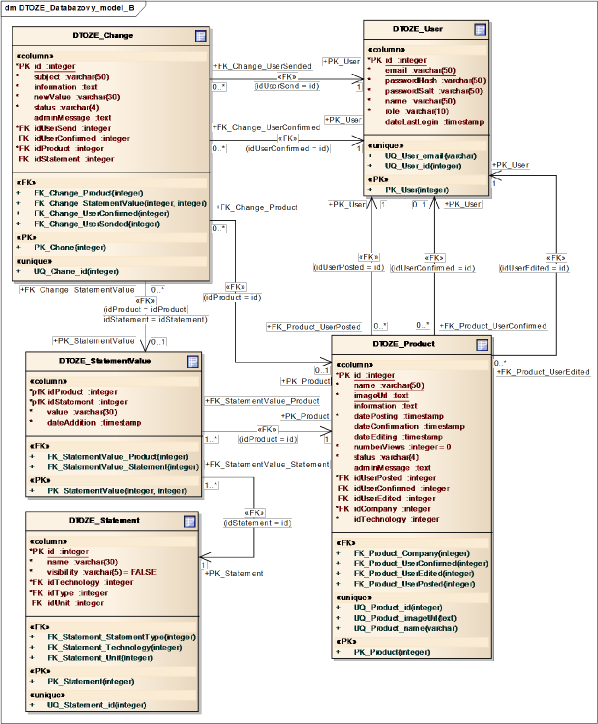
\includegraphics[scale=0.75]{DTOZE_fyzB_n} 
\label{fig:DTOZE_fyz_B}
\end{figure} 

Zatímco ER model by měl být srozumitelný jak pro zadavatele tak pro analytiky, databázový model musí přehledný především pro vývojáře, který nad ním implementuje aplikaci. Protože je dobrým zvykem psát kód v angličtině a z modelu bude generován SQL skript\footnote{Vysvětleno v následujícím odstavci.}, přeložila jsem veškeré názvy do angličtiny. Dále je před každým názvem uvedena prefix DTOZE, který jsem zavedla z bezpečnostního důvodu.\footnote{Vysvětleno v kapitole č.~\ref{cap:bezpecnost}.} Vztahy jsou vyjádřeny pomocí spojení přes cizí klíč. V závorkách jsou zobrazeny i sloupce, přes které je spojení realizováno. 

\begin{figure}[H] 
\centering 
\caption{Databázový model DTOZE C} 
\vspace{0.1cm}
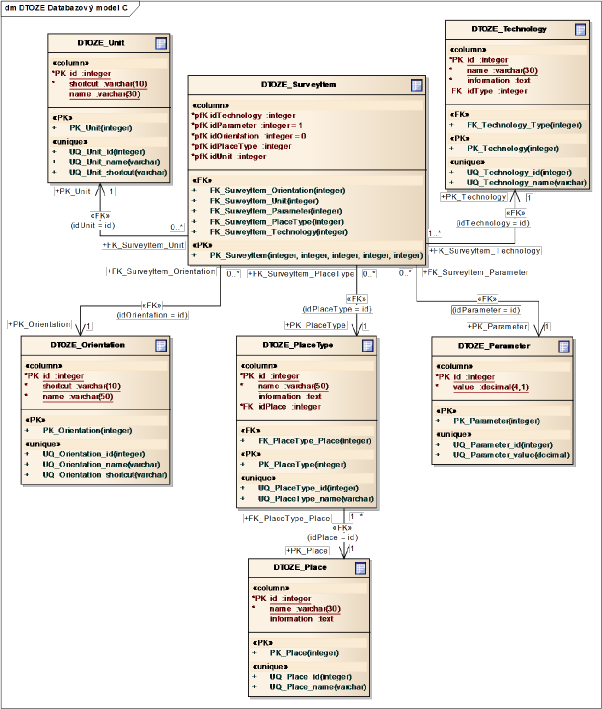
\includegraphics[scale=0.75]{DTOZE_fyzC_n} 
\label{fig:DTOZE_fyz_C}
\end{figure} 
\vspace{0.3cm}

Výhodou je, že modelovací nástroje většinou umožňují generovat SQL skript pro vytvoření tabulek včetně navolených datových typů a integritních omezení dle vybraného DBMS. Není nutné tedy ovládat SQL jazyk pro příkazy na vytvoření tabulek a integritních omezení, nicméně je vhodné je znát, jelikož se na vygenerovaný skript se nelze vždy spolehnout a je nutné jej ještě upravovat. Např. Enterprise Architect z databázového modelu DTOZE nevygeneroval dva cizí klíče a bylo je nutné doplnit. Dále je vhodné vygenerovaný skript upravit do logických celků, aby byl přehlednější (např. příkazy pro~vytvoření primárních klíčů je vhodné mít přímo u tabulky, které se nastavení týká, apod.) V~rámci práce se nebudu vysvětlení příkazů SQL věnovat podrobně, zmíním pouze základní příkazy pro vytvoření kompletní databáze, které jsou součástí SQL skriptu. 

Pro vytváření tabulek slouží v SQL příkaz CREATE TABLE. V rámci tohoto příkazu lze nastavit veškeré vlastnosti tabulky - sloupce a omezení sloupců včetně primárních a cizích klíčů. Omezení lze pojmenovat, a je to doporučeno z důvodu pozdější změny či vymazání omezení. Pro vytvoření unikátních hodnot, primárních a cizích klíčů proto je použit příkaz ALTER TABLE ve spojení s~příkazem ADD CONSTRAINT. Ukázka vytvoření jedné z tabulek znázorňuje následující úryvek kódu v jazyce SQL pro databázový systém PostgreSQL.   

\begin{lstlisting}[language=SQL, label=DescriptiveLabel, backgroundcolor=\color{grey}, numbers=left, basicstyle=\footnotesize]
CREATE TABLE DTOZE_Statement ( 
	id integer NOT NULL,
	name varchar(50) NOT NULL,
	idTechnology integer NOT NULL,
	idStatementType integer NOT NULL,
	idUnit integer
);

CREATE SEQUENCE statement_id_seq;

ALTER TABLE DTOZE_Statement ALTER id SET DEFAULT NEXTVAL('statement_id_seq');

ALTER TABLE DTOZE_Statement
	ADD CONSTRAINT UQ_Statement_id UNIQUE (id);

ALTER TABLE DTOZE_Statement
	ADD CONSTRAINT UQ_Statement_name UNIQUE (name);

ALTER TABLE DTOZE_Statement ADD CONSTRAINT PK_Statement 
	PRIMARY KEY (id);
\end{lstlisting}
\vspace{0.5cm}

V rámci sloupců a tabulek lze definovat i omezení CHECK. Toto omezení před vložením dat do~databáze zkontroluje podmínku pro vložení. Této podmínky lze využít v rámci jednoho, ale i více sloupců tabulky. Použití opět demonstruji na části SQL skriptu DTOZE. Omezení valide\_mail kontroluje pomocí regulárního výrazu správný formát e-mailu. Omezení non\_empty\_message kontroluje zda není zpráva prázdná. 

\vspace{0.5cm}
\begin{lstlisting}[language=SQL, label=DescriptiveLabel, backgroundcolor=\color{grey}, numbers=left, basicstyle=\footnotesize]
ALTER TABLE DTOZE_Application ADD CONSTRAINT valide_email 
  CHECK (email ~ '^[A-Za-z0-9._%-]+@[A-Za-z0-9.-]+[.][A-Za-z]{2,6}$');
  
ALTER TABLE DTOZE_Change
  ADD CONSTRAINT non_empty_message CHECK (adminMessage <> '');
\end{lstlisting}
\vspace{0.5cm}

V rámci definování vztahů a atributů jsem narazila i na několik omezení, která nelze definovat pouze v rámci sloupců či tabulek. Tato omezení lze také implementovat v rámci podmínky CHECK, jelikož lze v rámci omezení CHECK použít i uživatelsky definované funkce, kde lze pracovat s daty pomocí jazyka SQL. Ty se vytváří pomocí příkazu CREATE FUNCTION, v případě použítí v CHECK musí vracet typ BOOLEAN\footnote{Hodnotu TRUE nebo FALSE dle vyhodnocení těla funkce.}. Definice a použití funkce znázorňuji v následujícím úryvku kódu.

\newpage
\vspace{0.5cm}
\begin{lstlisting}[language=SQL, label=DescriptiveLabel, backgroundcolor=\color{grey}, numbers=left, basicstyle=\footnotesize, breaklines=true, breakatwhitespace=true, showspaces=false, showstringspaces=false]
CREATE OR REPLACE FUNCTION check_user_role(INTEGER) RETURNS BOOLEAN AS '
DECLARE
    tmpRole VARCHAR(10);
BEGIN
SELECT role INTO tmpRole FROM DTOZE_user WHERE id = $1;      
     IF FOUND THEN
      RETURN (tmpRole LIKE ''producent'');
     ELSE 
      RETURN false;
     END IF;
 END;
' LANGUAGE plpgsql;

ALTER TABLE DTOZE_Company ADD CONSTRAINT valide_user 
  CHECK (check_user_role(idProducent));
\end{lstlisting}
\vspace{0.5cm}

Otázkou stále zůstává, zda je kontrola na databázové vrstvě ve vícevrstvých aplikacích užitečná. V~případě, že v se v rámci aplikace někdo pokusí o vložení nějakých dat a nad daty vyjde v podmínce CHECK FALSE, databázový systém vyhodí výjimku, která ale v aplikaci nebude znázorněna (pokud to nebude implementováno) a uživatel se nedozví, že se jeho záznam neuložil. Proto je nutné data kontrolovat už na vyšších vrstvách, aby bylo zaručeno, že budou např. ve správném formátu a pokud ne, dostane uživatel upozornění ještě před tím, než se k databázi přistoupí. Domnívám se, že omezení CHECK je pro použití v DTOZE zbytečné. V SQL skriptu proto budou uvedeny pouze ukázkové příklady. 

\subsubsection{Návrh odvozených sloupců} 
Při konceptuálním návrhu dat bylo možné definovat tzv. odvozené atributy. Jedná se o atributy, jejichž hodnota je odvozená (nejčastěji vypočítaná) z jiných atributů či tabulek. Nejčastěji se jedná o počty v~rámci vztahů mezi entitami. Tyto atributy lze realizovat pomocí odvozených sloupců. Tyto sloupce je v tabulce nutné udržovat, aby stále obsahovaly aktuální informace, za cenu jednoduchého dotazování.

K tomu slouží v DBMS tzv. triggery\footnote{Triggery slouží i k operacím, které je nutné provést v rámci jedné transakce, viz další kapitola.} neboli spouštěče. Ty provedou požadovanou akci nad daným sloupcem či více sloupci nebo nad jednou či více tabulkách a to buď při vkládání, upravování či mazání. Trigger se skládá ze tří částí: událost nebo události, které spustí trigger (např. INSERT, UPDATE, DELETE nebo i CREATE, ALTER, DROP a další); podmínka, která určuje, za jakých okolností má být trigger spuštěn; akce, která se vykoná po splnění podmínky. Trigger lze definovat na úrovni řádku, ale i na úrovni pouze příkazu. Zatímco trigger definovaný na úrovni řádku se spustí pro všechny řádky, kterých se týká spouštěcí událost, trigger na úrovni příkazu se provede pouze jednou.Trigger se vytvoří příkazem CREATE TRIGGER a v rámci vytváření triggeru lze používat již dříve definované funkce.\footnote{CONOLLY, Thomas, Carolyn BEGG a Richard HOLOWCZAK. \textit{Mistrovství - databáze: profesionální průvodce tvorbou efektivních databází}. Vyd. 1. Brno: Computer Press, 2009, 584 s. ISBN 978-80-251-2328-7. Str. 508-509.}  

V původním návrhu DTOZE se nevyskytují žádné odvozené sloupce, jelikož jsem počítala s tím, že je nepoužiji. Nyní jsem ale situaci přehodnotila. Některé odvozené sloupce by bylo vhodné doimplementovat, místo neustálého přepočítávání. Např. je to vhodné pro veškeré statistiky. Zavedené změny je důležité zavést do všech diagramů a vytvořit příslušné triggery pomocí SQL. Změny v návrhu DTOZE jsou k~zhlédnutí v přílohách, kde jsou uvedeny finální modely ze všech fází návrhu - ER model je přílohou~\ref{attach:DTOZE-ER}, logický model přílohou~\ref{attach:DTOZE-log} a databázové model přílohou~\ref{attach:DTOZE-dt}. Implementaci triggeru použitého v~DTOZE znázorňuje následující kód v jazyce SQL pro databázový systém PostgreSQL. Trigger po přidání, smazání nebo upravování nového produktu do databáze upraví odvozené sloupece v~tabulkách DTOZE\_User, DTOZE\_Company a DTOZE\_Technology. Je však nutné brát ohled na~to, že se produkt může nacházet v několika různých stavech (OK, KO, WAIT). V případě, že není produkt ve~stavu OK, nepočítá se s ním v uložených hodnotách, jelikož častěji bude potřeba znát počet produktů ve~stavu OK, než celkový počet v databázi. 

\vspace{0.3cm}
\begin{lstlisting}[language=SQL, label=DescriptiveLabel, backgroundcolor=\color{grey}, numbers=left, basicstyle=\tiny, breaklines=true, breakatwhitespace=true, showspaces=false, showstringspaces=false]
CREATE OR REPLACE FUNCTION update_productCounters() RETURNS TRIGGER AS '
BEGIN
    IF TG_OP = ''DELETE'' THEN
        IF OLD.status LIKE ''OK'' THEN
          UPDATE DTOZE_User SET countProductPosted = countProductPosted - 1 WHERE id = OLD.idUserPosted;
          UPDATE DTOZE_Company SET countProduct = countProduct - 1 WHERE id = OLD.idCompany;
          UPDATE DTOZE_Technology SET countProduct = countProduct - 1 where id = OLD.idTechnology;
        END IF;
        RETURN OLD;
    END IF;
    IF TG_OP = ''INSERT'' THEN
        IF NEW.status LIKE ''OK'' THEN
          UPDATE DTOZE_User SET countProductPosted = countProductPosted + 1 WHERE id = NEW.idUserPosted;
          UPDATE DTOZE_Company SET countProduct = countProduct + 1 WHERE id = NEW.idCompany;
          UPDATE DTOZE_Technology SET countProduct = countProduct + 1 where id = NEW.idTechnology;
        END IF;
        RETURN NEW;
    END IF;
    IF TG_OP = ''UPDATE'' THEN
        IF (OLD.status LIKE ''OK'' AND NEW.status LIKE ''OK'') THEN
          IF (OLD.idUserPosted != NEW.idUserPosted) THEN
            UPDATE DTOZE_User SET countProductPosted = countProductPosted + 1 WHERE id = NEW.idUserPosted;
            UPDATE DTOZE_User SET countProductPosted = countProductPosted - 1 WHERE id = OLD.idUserPosted; 
          END IF;
          IF OLD.idCompany != NEW.idCompany THEN
            UPDATE DTOZE_Company SET countProduct = countProduct + 1 WHERE id = NEW.idCompany;
            UPDATE DTOZE_Company SET countProduct = countProduct - 1 WHERE id = OLD.idCompany;
          END IF;
          IF OLD.idTechnology != NEW.idTechnology THEN
            UPDATE DTOZE_Technology SET countProduct = countProduct + 1 where id = NEW.idTechnology;
            UPDATE DTOZE_Technology SET countProduct = countProduct - 1 where id = OLD.idTechnology;
          END IF;
        ELSEIF (OLD.status NOT LIKE ''OK'') AND (NEW.status LIKE ''OK'') THEN
          UPDATE DTOZE_User SET countProductPosted = countProductPosted + 1 WHERE id = NEW.idUserPosted;
          UPDATE DTOZE_Company SET countProduct = countProduct + 1 WHERE id = NEW.idCompany;
          UPDATE DTOZE_Technology SET countProduct = countProduct + 1 where id = NEW.idTechnology;
        ELSEIF (OLD.status LIKE ''OK'') AND (NEW.status NOT LIKE ''OK'') THEN
          UPDATE DTOZE_User SET countProductPosted = countProductPosted - 1 WHERE id = OLD.idUserPosted;
          UPDATE DTOZE_Technology SET countProduct = countProduct - 1 where id = OLD.idTechnology;
          UPDATE DTOZE_Company SET countProduct = countProduct - 1 WHERE id = OLD.idCompany;
        END IF;
        RETURN NEW;
    END IF;
END;
' LANGUAGE 'plpgsql';

CREATE TRIGGER TGR_update_productCounters
AFTER INSERT OR DELETE OR UPDATE ON DTOZE_Product
FOR EACH ROW EXECUTE PROCEDURE update_productCounters();
\end{lstlisting}
\vspace{0.3cm}
\newpage

\subsubsection{Analýza transakcí}
Pro bezpečné ukládání a čtení dat je velmi důležité, aby veškeré operace byly atomické, konzistentní, izolované a stálé. Tyto problémy řeší DBMS pomocí transakcí - jednoho či několika SQL příkazů, které se vykonávají najednou. Atomicitou je myšleno, že transakce musí proběhnout celá a nebo neproběhnout vůbec. V rámci konzistence nesmí dojít k situaci, že během provádění jedné transakce ovlivňuje data ke zpracování jiná transakce. S tím souvisí i izolovanost, neboli změny provedené před potvrzením transakce musí být izolovány před ostatními transakcemi. Poslední vlastností je stálost, tedy po~potvrzení transakce musí být databáze opět v konzistentním stavu a to neustále.\footnote{Tyto vlastnosti nesou název ACID, dle prvních písmen těchto vlastností v anglickém jazyce - atomicity, consistency, isolation, durability.} \footnote{Teorie databází: Transakce. \textit{www.manualy.net} [online]. 22. 12. 2005 [cit. 2014-05-09]. Dostupné z: \url{http://www.manualy.net/article.php?articleID=8}.}

O to, aby transakce probíhali správně, se z velké části stará DBMS, některé případy je však nutné ošetřit dodatečně. Pro jeden příkaz do databáze DBMS obvykle vytvoří samostatnou transakci. U~některých skupin příkazů je to ale nežádoucí. Např. při převodu peněz z jednoho účtu na druhý je nutné zkontrolovat, zda má odesílatel dostatek peněz, poté odesílateli strhnout peníze a zároveň příjemci účet navýšit o poslanou částku. V případě, že by se v oddělené transakci peníze odečítali, v jiné přičítali a mezitím spadl systém, z jednoho účtu se peníze přičtou a na druhém neodečtou. Takových případů může nastat několik. 

Proto je nutné takové případy v databázi najít a zdokumentovat a popřípadě ošetřit pomocí nástrojů DBMS (např. pomocí zmiňovaných triggerů či úložných procedur), nebo jinými způsoby dle implementace. Dále je vhodné analyzovat i nejpoužívanější transakce a odhadnout průměrný a maximální počet provedení za hodinu/den, popř. rozmezí hodin, kdy je vytížení největší. Tyto informace dále poslouží při zefektivňování databázového návrhu. 

U návrhu DTOZE jsem nenalezla žádné nebezpečné operace, které by bylo nutné provádět v rámci jedné transakce. Tabulka č. \ref{fig:DTOZE_fyz_analyza} znázorňuje analýzu transakcí provedenou nad DTOZE. 
\vspace{0.5cm}
\begin{table}[H] 
\centering 
\caption{Analýza transakcí nad DTOZE} 
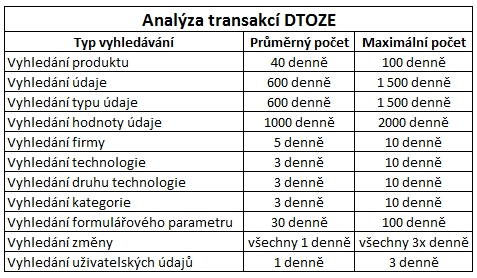
\includegraphics[scale=0.6]{DTOZE_fyz_analyza} 
\label{fig:DTOZE_fyz_analyza}
\end{table} 
\vspace{0.5cm}

\subsubsection{Indexování}
Při návrhu databáze se při konceptuálním a logickém návrhu klade důraz na to, aby byla data správně uložena - nedocházelo k redundanci a byla snadno editovatelná. Ve fyzickém návrhu je důležité se zaměřit i na to, aby se k datům přistupovalo rychle a efektivně.

V databázovém systému lze krom vytvoření tabulek a integritních omezení nastavit i tzv. indexování. Data se do databáze ukládají do tabulek většinou postupně za sebe. V případě, že je nutné najít nějaká data, která splňují zadané kritérium, musí se projít celá tabulka a u všech záznamů kontrolovat, zda nesplňují toto kritérium. K tomu, aby se nemusely všechny záznamy procházet, slouží v DBMS indexy. „Index je datová struktura, která umožňuje DBMS rychleji lokalizovat konkrétní záznamy v~souboru, a~tak zrychlit odezvu na uživatelské dotazy.“\footnote{CONOLLY, Thomas, Carolyn BEGG a Richard HOLOWCZAK. \textit{Mistrovství - databáze: profesionální průvodce tvorbou efektivních databází}. Vyd. 1. Brno: Computer Press, 2009, 584 s. ISBN 978-80-251-2328-7. Str. 511.} Index je seřazený a každá položka indexu odkazuje na požadovanou položku a jeden nebo více údajů o její lokalizaci.\footnote{Tamtéž str. 511.}

Indexy lze vytvářet nad jedním nebo několika sloupci tabulky a každá tabulka může mít několik indexů. Index definovaný nad sloupcem tabulky pak umožní rychlý přístup k datům podle hodnot sloupce. Existuje několik typů indexů. Speciální index má automaticky např. sloupec s primárním klíčem či sloupec s omezením UNIQUE\footnote{Jedná se o omezení zaručující unikátnost sloupce.}. Dále lze vytvořit tzv. sekundární index. Takový index umožňuje např. rychlé seřazení tabulky podle sloupců, nad kterými je index definován.\footnote{VRÁNA, Jakub. Využití databázových indexů. \textit{Root.cz} [online]. 22. 7. 2003 [cit. 2014-04-09]. Dostupné z: \url{http://www.root.cz/clanky/vyuziti-databazovych-indexu/}.} Např. u tabulky DTOZE\_Product se díky primárnímu klíči bude přistupovat především pomocí indexu nad primárním klíčem. Ale jelikož se v rámci aplikace budou produkty nejčastěji vypisovat podle data schválení či data poslední změny, je vhodné nad těmito sloupci vytvořit sekundární index.

Indexy jsou u tabulek s méně než stovkami záznamů téměř zanedbatelné. Naopak databázový systém je zatěžován udržováním indexů. U větších tabulek však můžou výrazně zefektivnit přístup k datům.\footnote{Tamtéž.} Při vytváření indexů je vhodné vycházet z analýzy transakcí, kde jsou popsány často prováděné transakce, či transakce kriticky důležité pro chod aplikace. Dále je vhodné definovat index pro cizí klíče, přes které se často spojují tabulky.\footnote{VONDRA, Tomáš. Obvyklé problémy s SQL: indexy. \textit{fuzzy.cz: Because the world is not a crisp...} [online]. 4. 8. 2009 [cit. 2014-04-09]. Dostupné z: \url{http://www.fuzzy.cz/cs/clanky/obvykle-problemy-s-sql-indexy/}.}

Pro DTOZE jsem se rozhodla vytvořit sekundární index u zmiňované tabulky DTOZE\_Product (nad sloupci dateConfirmation, dateEditing, numberViews) a u tabulky DTOZE\_Company (nad sloupcem numberViews). Dále jsem vytvořila index nad cizími klíči tabulek, které budou obsahovat nejvíce záznamů a budou často spojovány přes cizí klíč - týká se tabulky DTOZE\_Product a DTOZE\_Statement. K ostatním tabulkám se bude přistupovat nejčastěji přes primární klíč. Implementaci jednoho ze zmiňovaných indexů znázorňuje následující úryvek kódu v jazyce SQL pro databázový systém PostgreSQL.  

\vspace{0.3cm}
\begin{lstlisting}[language=SQL, label=DescriptiveLabel, backgroundcolor=\color{grey}, numbers=left, basicstyle=\footnotesize]
CREATE INDEX IX_Product_idCompany
	ON DTOZE_Product (idCompany);
\end{lstlisting}
\vspace{0.3cm}

\subsubsection{Návrh pohledů}
Jazyk SQL umožňuje krom vytváření tabulek definovat struktury tabulkám podobné, ale ve své podstatě naprosto odlišné - pohledy. Pohled je struktura, ke které lze přistupovat jako k tabulkám (tedy lze z pohledu data číst, vkládat, mazat), avšak plnohodnotnými tabulkami nejsou. Jedná se totiž pouze o pojmenovaný SQL dotaz, který vybírá konkrétní sloupce pro další čtení či upravování. Nezabírá tedy žádné místo. Pohledy lze vytvořit buď z jedné tabulky (např. zredukováním sloupců), nebo spojením více tabulek (např. spojení tabulek, které je často používáno).

Pohledy lze použít především pro zpřehlednění dotazů, nebo pro dotazy, které by se jinak často opakovaly. Zásadní význam ale mohou mít i při zabezpečování databáze. Pokud do databáze přistupuje fyzicky více uživatelů s různými pravomocemi, lze pomocí pohledů omezit přístup k některým sloupcům či k celým tabulkám. 

Aplikace nad DTOZE bude implementována pomocí objektově relačního mapování (ORM). K tabulkám se bude přistupovat pomocí objektů, které budou namapovány na tabulky. K datům se nebude přistupovat pomocí SQL (v některých případech to bude nutné), ale jinými mechanismy. Nemyslím si tedy, že jsou pohledy konkrétně pro DTOZE užitečné. Avšak je vhodné tuto funkčnost znát a v případě nutnosti implementovat. Na~ukázku uvádím pohled vytvořený nad tabulkami DTOZE\_Statement a~DTOZE\_Unit, který spojuje tyto tabulky, a v případě nepoužití ORM by měl velký význam, jelikož hodnoty údaje a jednotky budou vždy zobrazovány společně. Pohledy též nejsou součástí SQL skriptu DTOZE. Implementaci pohledu znázorňuje následující úryvek kódu v jazyce SQL pro databázový systém PostgreSQL.

\vspace{0.5cm}
\begin{lstlisting}[language=SQL, label=DescriptiveLabel, backgroundcolor=\color{grey}, numbers=left, basicstyle=\footnotesize, breaklines=true, breakatwhitespace=true]
CREATE VIEW full_statement AS
 SELECT DTOZE_Statement.id, DTOZE_Statement.name, DTOZE_Statement.visibility, DTOZE_Unit.shortcut
 FROM DTOZE_Statement AS s, DTOZE_Unit AS u
 WHERE s.id = u.id;
\end{lstlisting}
\vspace{0.5cm}

\subsubsection{Zohlednění denormalizace \label{cap:denormalizace}}
V rámci logického návrhu jsem se zabývala normalizací tabulek. Týkala se sloupců jednotlivých tabulek. Cílem bylo zamezit redundanci a zajistit snadné editování dat. Tabulky jsem rozdělila a svázala pomocí cizích klíčů. Takové rozdělení tabulek může být z hlediska redundace vhodné, ale z hlediska efektivnímu přistupování k datům občas nevhodné. 

Proto v rámci fyzického návrhu může dojít ještě k přezkoumání tabulek a následné denormalizaci dle potřeb. Denormalizace by se především měla týkat databáze, která svým návrhem nesplňuje požadavky na výkonnost. Tedy týká se to především aplikací, které pracují s velkým množstvím\footnote{Odhadem v řádech miliónů a více záznamů.} dat. Hlavními výhodami denormalizace je minimalizace potřeby spojení tabulek, snížení počtu cizích klíčů v tabulkách, snížení počtu indexů a počtu tabulek. Nevýhodami je naopak zpomalení aktualizace dat a může zvětšit velikost tabulek. Další nevýhodou je, že se vztahuje ke konkrétní aplikaci, je na to tedy nutné brát zřetel. Dále může v některých případech zhoršit implementaci a flexibilita.\footnote{CONOLLY, Thomas, Carolyn BEGG a Richard HOLOWCZAK.\textit{Mistrovství - databáze: profesionální průvodce tvorbou efektivních databází}. Vyd. 1. Brno: Computer Press, 2009, 584 s. ISBN 978-80-251-2328-7. Str. 278.} V případě upravení tabulek je nutné se vrátit k předchozímu kódu a dle změn upravit omezení či indexování.

V rámci normalizace DTOZE jsem již porušila některé normy z důvodu efektivnějšího přístupu k datům a denormalizaci již praktikovala (u tabulky DTOZE\_Company). Denormalizaci bych například mohla uvážit i u několikanásobného vztahu mezi DTOZE\_Technology, DTOZE\_Orientation, DTOZE\_PlaceType, DTOZE\_Unit a DTOZE\_Parameter, které jsou spojené pomocí vztahové tabulky DTOZE\_SurveyItem. Pro získání celistvé informace je nutné spojit pět tabulek. Jelikož je ale dat v jednotlivých tabulkách málo (max. 10 záznamů), lze tyto tabulky spojit rovnou v jednu, za~cenu redundance dat. Jak znázorňuje obrázek č. \ref{fig:DTOZE_fyz_CD_denormalizace}. (Čitelnější původní diagram před denormalizací je samostatně na obrázku č.~\ref{fig:DTOZE_fyz_C}.) 

\begin{figure}[H] 
\centering 
\caption{Ukázka denormalizace na DTOZE} 
\vspace{0.2cm}
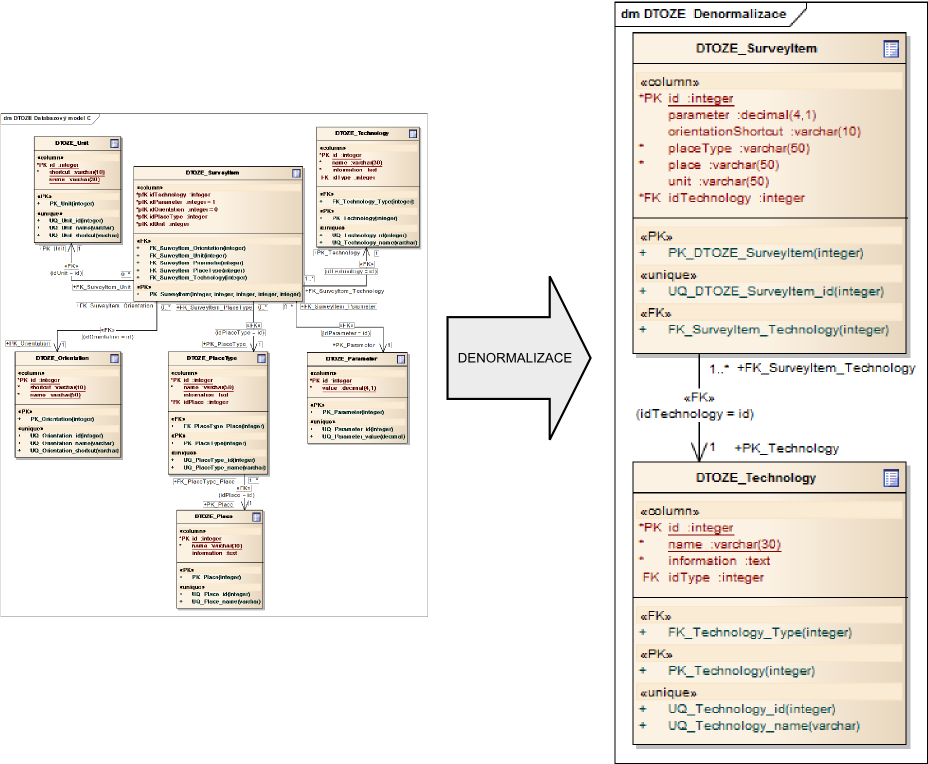
\includegraphics[scale=0.55]{DTOZE_fyzCD_denormalizace_n} 
\label{fig:DTOZE_fyz_CD_denormalizace}
\end{figure} 

Jelikož předpokládaný počet záznamů v DTOZE nepřesáhne celkově za rok fungování databáze více jak 100~000~záznamů a předpokládaný růst po roce užívání je velmi malý, uvažuji, že požadavky na výkon budou bez problémů splněny, není tedy nutné se denormalizací v rámci DTOZE zabývat.  

\subsubsection{Návrh bezpečnostních opatření \label{cap:bezpecnost}}
Návrh bezpečnostních opatření se týká především vytvoření pohledů pro jednotlivé uživatele databáze. Jelikož bude přístup do databáze všem uživatelům umožněn pouze přes uživatelské rozhraní, není potřeba uživatelské pohledy implementovat. Přímý přístup k tabulkám DTOZE bude mít pouze aplikace a správce serveru přes uživatelské jméno a heslo. 

Nad rámec běžného zabezpečení jsem uvažovala i různé útoky na zabezpečení aplikace. Např. není vhodné pojmenovávat tabulky snadno odhadnutelnými názvy, jako je např. Users. Vhodné je doplnit názvy např. prefixem, který mají všechny tabulky společné (např. DTOZE\_User). V případě proniknutí přes zabezpečení aplikace lze poté snadno odhalit, kde se nacházejí citlivé informace, které lze takto snadno získat. Avšak toto nezajistí ukradení dat, pouze jej může zbrzdit. Přednostně je nutné v rámci zabezpečení celé aplikace zajistit, aby se k datům v databázi nebylo možné dostat jinak, než je žádoucí. Prefix je ale vhodný i z důvodu rozšiřování aplikace. V případě, že by nějaká aplikace přistupovala k~více databázím, je jednoznačně určeno, které tabulky patří do jaké databáze.

\subsubsection{Testování SQL skriptu}
V rámci fyzického návrhu byl SQL skript několikrát modifikován. Byla doplněna nová omezení či dotvořené funkce či triggery. Během vytváření nových funkčností bylo průběžně testováno, zda je na zavedené operace očekávaná odpověď a zda jsou všechny příkazy syntakticky správně.  

Funkčnost je sice zkontrolována, ale je vhodné ji ještě ověřit i v rámci hodnot v tabulkách. Proto je potřeba do vytvořených tabulek vložit testovací data a ověřit správnou provázanost systému na konkrétních hodnotách. Pro vkládání dat do databáze je příkaz INSERT INTO, pro upravování UPDATE a pro mazání DELETE. Již v rámci vkládání dat lze najít chyby např. v definovaných omezení. Upravováním a mazáním dat lze zkontrolovat fungování triggerů např. na odvozených sloupcích, zda mění hodnoty správně. Výsledný skript je také vhodné komentovat pro další uživatele, kteří s ním budou pracovat. Finální SQL skript pro vytvoření DTOZE je přílohou \ref{attach:DTOZE-skript}.    


\newpage
\section{Závěr}
V úvodu práce byla provedena rešerše aplikací na Internetu zabývajících se podobnou tématikou. Dále byly popsány požadavky na databázi, konkrétně databázi technologií využívajících obnovitelné zdroje energie pro drobné investory, a navrhnuty výpočty pro hodnocení investice do zařízení využívajících OZE. Celá databáze byla navrhnuta dle metodiky, která byla detailně vysvětlena a demonstrována na konkrétním zadání. 

Hlavním cílem práce bylo navrhnout databázi dle požadavků. Cíl práce se podařil naplnit, zároveň byly zohledněny požadavky na webovou aplikaci, která bude vytvořena nad databází. Výsledkem je dokumentace návrhu databáze a funkční SQL skript pro fyzické vytvoření databáze na serveru. Cílem práce bylo také popsat srozumitelně metodiku návrhu relační databáze. V rámci práce vznikl stručný návod, který shrnuje postup při návrhu databáze pro různé aplikace. Snahou bylo popsat veškeré případy, na které lze při návrhu databáze narazit, což se výběrem nepříliš snadného zadání podařilo naplnit. Tento manuál dále plánuji zpřístupnit online.  

Při vytváření návrhu byl největší problém se správným definováním požadavků. Nejdříve jsem definovala požadavky na databázi velmi stručně, nevytvořila jsem detailní popis a začala tvořit návrh. Při zpětném kontrolování, zda model uchovává všechny informace, včetně těch, které nejsou popsány, ale budou důležité při implementaci, jsem narazila na mnoho nesrovnalostí. Musela jsem se vrátit k~požadavkům a definovat je konkrétněji. Při detailním promýšlení případů užití jsem již myslela i~na implementaci a propojila vše dohromady. Celý návrh jsem pak ale musela předělat s ohledem na změny, které nebyly malé. Při příštím návrhu tedy tuto část nepodcením a více se na ní zaměřím.

Dalším krokem navazujícím na práci je rozšíření dokumentace projektu a následně implementace webové aplikace nad vzniklou databází. Možností jak rozšířit v budoucnu vzniklou aplikaci je několik. Jedním z požadavků, které nebyly zahrnuty do návrhu, je rozšíření verze z českého jazyka i do jazyka anglického. A to z prostého důvodu - většina výrobců je ze zahraničí. Databáze by se tak mohla více rozrůstat. Dále je to možnost zveřejňování článků s tématikou drobných technologií využívající OZE, které by pomohly rozšiřovat povědomí o problematice OZE a upozorňovat na zajímavosti. Dalším nezahrnutým požadavkem je propojení s metadaty geoinformačních vrstev České republiky (mapou iradiace, větrnou mapou apod.) v rámci projektu RESTEP (Regional Sustainable Energy Policy) a~upravení návrhu vhodného řešení s ohledem na data z těchto map. Na tyto plány bude brán zřetel při navázání na práci.

\newpage
\section{Seznam zdrojů}
\begin{enumerate}
\item  BECHNÍK, Bronislav. Fotovoltaika jako náhrada biopaliv v dopravě. \textit{tzbinfo.cz: stavebnictví, úspory energií, technická zařízení budov} [online]. 2. 9. 2013 [cit. 2014-04-12]. Dostupné z: \url{http://oze.tzb-info.cz/fotovoltaika/10291-fotovoltaika-jako-nahrada-biopaliv-v-doprave}.
\item CONOLLY, Thomas, Carolyn BEGG a Richard HOLOWCZAK. \textit{Mistrovství - databáze: profesionální průvodce tvorbou efektivních databází.} Vyd. 1. Brno: Computer Press, 2009, 584 s. ISBN 978-80-251-2328-7.
\item Daze.vukoz.cz. VÝZKUMNÝ ÚSTAV SILVA TAROUCY PRO KRAJINU A~OKRASNÉ ZAHRADNICTVÍ, veřejná výzkumná instituce. \textit{DAZE: Databáze obnovitelných zdrojů energie} [online]. 2005 [cit. 2013-12-10]. Dostupné z: \url{http://daze.vukoz.cz/daze/index.jsp}.
\item Envisluzby.cz. CEMC. \textit{Databáze enviromentálních služeb a výrobků} [online]. 2011 [cit. 2013-12-10]. Dostupné z: \url{http://www.envisluzby.cz/}. 
\item HERNANDEZ, Michael J. a HOLOWCZAK. \textit{Návrh databází}. 1. vydání. Praha: Grada, 2006, 408 s. Profesional. ISBN 80-247-0900-7.
\item Hodnocení investic: Vnitřní výnosové procento (IRR).  \textit{BussinesVize.cz} [online]. 9. 11. 2010 [cit. 2014-04-12]. Dostupné z: \url{http://www.businessvize.cz/rizeni-a-optimalizace/hodnoceni-investic-vnitrni-vynosove-procento-irr}.
\item KNÁPEK, Jaroslav, Oldřich STARÝ a Jiří VAŠÍČEK. Zásady hodnocení ekonomické efektivnosti energetických projektů. \textit{Metodika EFEKT} [online]. 2003 [cit. 2014-04-12]. Dostupné z: \url{http://efekt.xf.cz/metodikaEFEKT.pdf}.
\item KULHAN, Jakub. Normalizace relačních databází. \textit{Programujte.com} [online]. 2008 [cit. 2013-12-10]. Dostupné z: \url{http://programujte.com/clanek/2008071900-normalizace-relacnich-databazi/}.
\item Res-legal.eu. EUROPEAN COMISSION. \textit{Renewable energy policy database and support} [online]. 2012 [cit. 2013-12-10]. Dostupné z: \url{http://www.res-legal.eu/}. 
\item Rešerše. \textit{Ústřední knihovna ČVUT} [online]. [cit. 2013-12-10]. Dostupné z: \url{http://knihovna.cvut.cz/sluzby/reserse/co-je-reserse.html}.
\item Rešerše: modelový příklad postupu. \textit{Správa Univerzitního kampusu Masarykovy univerzity} [online]. [cit. 2013-12-10]. Dostupné z: \url{http://ukb.muni.cz/kuk/animace/eiz/Reserse/reserse_praxe.html}.
\item SKŘIVAN, Jaromír. Databáze a jazyk SQL. \textit{Interval.cz} [online]. 2000 [cit. 2013-12-10]. Dostupné z: \url{http://interval.cz/clanky/databaze-a-jazyk-sql/}.
\item Teorie databází: Transakce. \textit{www.manualy.net} [online]. 22. 12. 2005 [cit. 2014-04-09]. Dostupné z: \url{http://www.manualy.net/article.php?articleID=8}.
\item VONDRA, Tomáš. Obvyklé problémy s SQL: indexy. \textit{fuzzy.cz: Because the world is not a crisp...} [online]. 4. 8. 2009 [cit. 2014-04-09]. Dostupné z: \url{http://www.fuzzy.cz/cs/clanky/obvykle-problemy-s-sql-indexy/}.
\item VRÁNA, Jakub. Využití databázových indexů. \textit{Root.cz} [online]. 22. 7. 2003 [cit. 2014-04-09]. Dostupné z: \url{http://www.root.cz/clanky/vyuziti-databazovych-indexu/}.
\end{enumerate}
\newpage

\appendix 
\section{Seznam zkratek}
BCNF - Boyce-Coddova normální forma\\
CF - Cash Flow\\
CEMC - České ekologické manažerské centrum\\
DBDL – Database Definition Language\\
DBMS – Database Management System\\
DTOZE – databáze technologí využívajících obnovitelné zdroje energie\\
DPP - Discounted Payback Period\\
ER – Eentity Relation\\
ID - IDentification\\
IRR - Internal Rate of Return\\
NPV - Net Present Value\\
ORM - objektově relačního mapování\\
OZE – obnovitelné zdroje energie\\
PDF - Portable Document Format\\
PP - Payback Period\\
RES – Renewable Energy Sources\\
SQL - Structured Query Language\\
UML - Unified Modeling Language\\
VÚKOZ - Výzkumný ústav Silva Taroucy pro krajinu a okrasné zahradnictví\\
XML - Extensible Markup Language\\
1NF - první normální forma \\
2NF - druhá normální forma \\
3NF - třetí normální forma \\
4NF - čtvrtá normální forma\\
5NF - pátá normální forma

\newpage
\section{Vize DTOZE\label{attach:DTOZE-vize}}
Vize je dostupná v elektronické podobě na nosiči společně s elektronickou verzí práce pod názvem DTOZE\_vision\_v1.pdf. 

\section{Finální ER model \label{attach:DTOZE-ER}}

\begin{figure}[H] 
\centering  
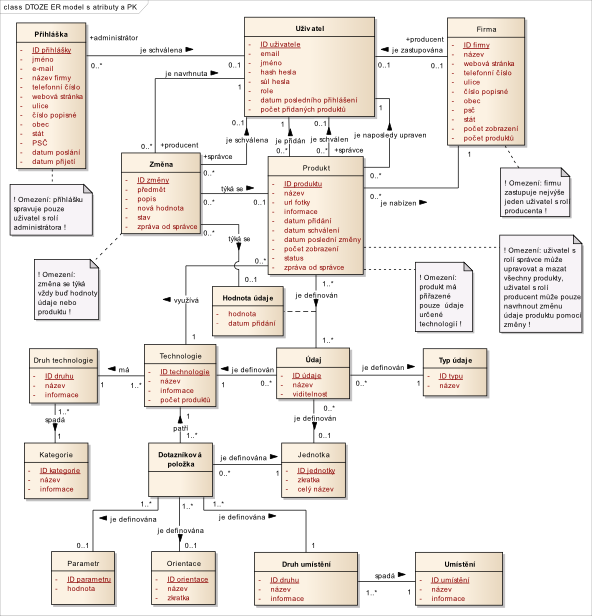
\includegraphics[scale=0.75]{DTOZE_ER_final_n} 
\end{figure} 

\section{Finální logický model\label{attach:DTOZE-log}}

\begin{table}[H] 
\centering  
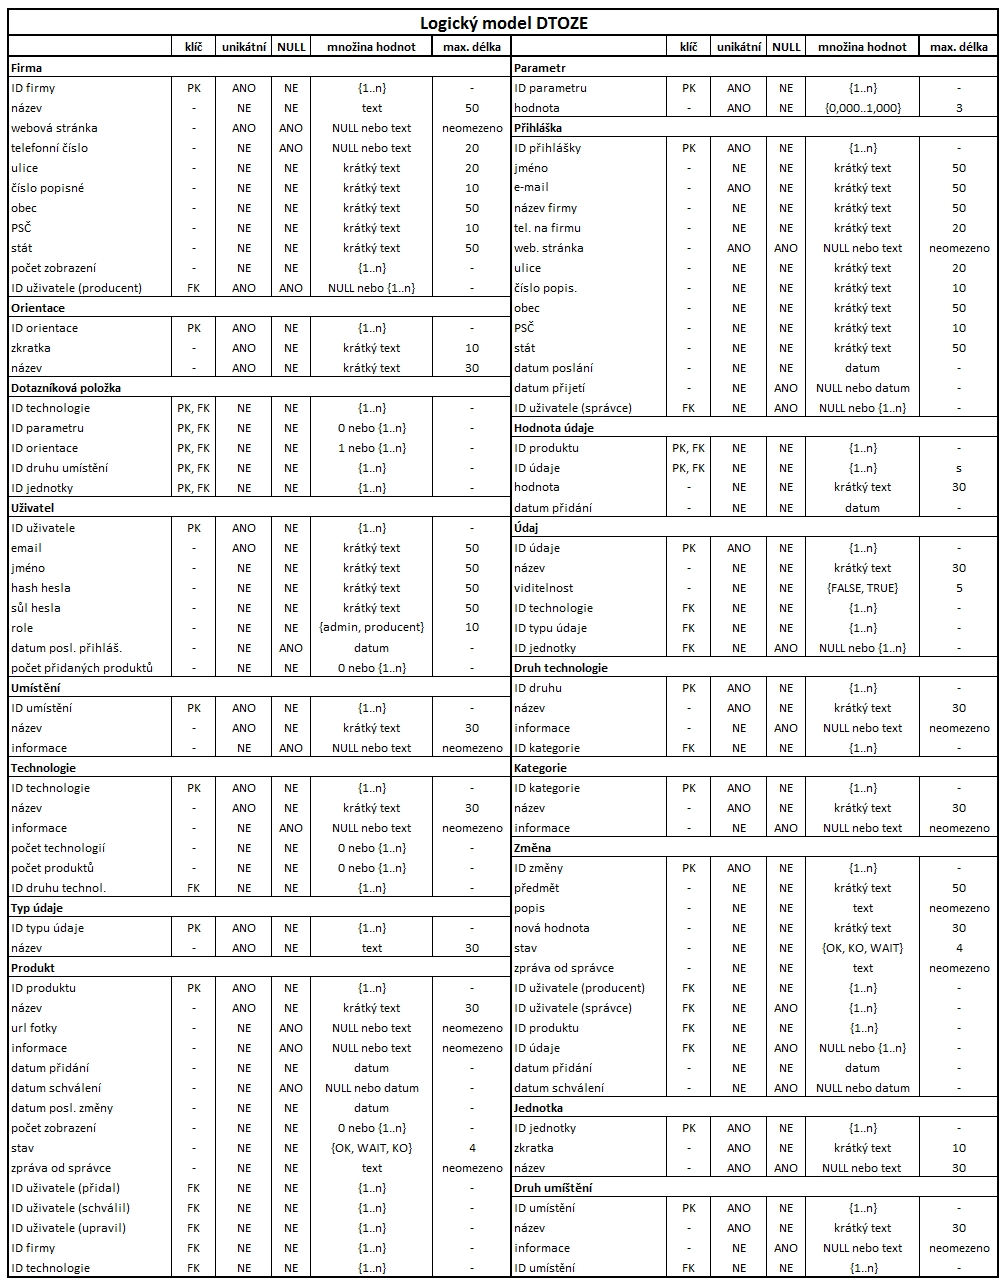
\includegraphics[scale=0.45]{DTOZE_log_D_final} 
\end{table}

\section{Finální databázový model\label{attach:DTOZE-dt}}

\begin{figure}[H] 
\centering  
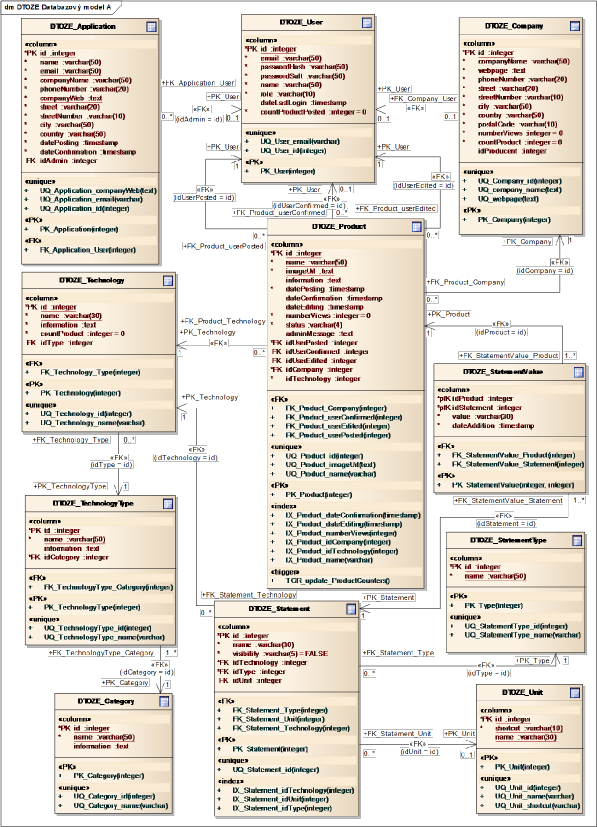
\includegraphics[scale=0.71]{DTOZE_fyzA_final_n} 
\end{figure}

\begin{figure}[H] 
\centering  
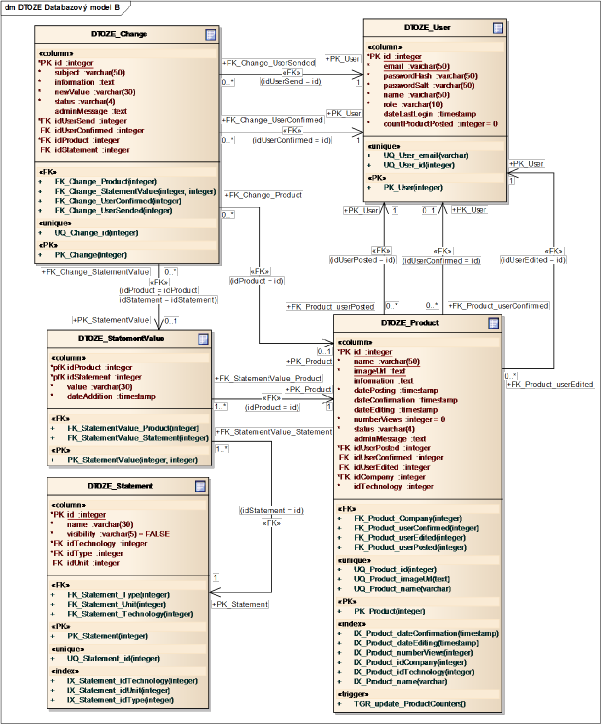
\includegraphics[scale=0.75]{DTOZE_fyzB_final_n} 
\end{figure}

\begin{figure}[H] 
\centering  
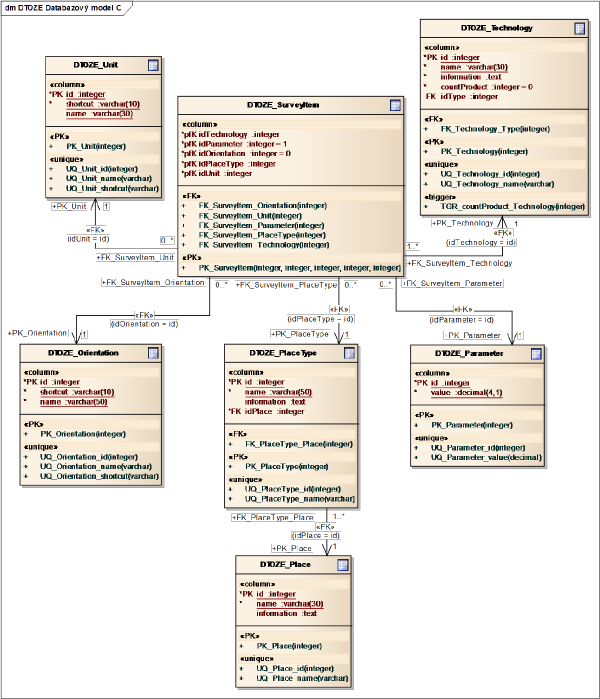
\includegraphics[scale=0.75]{DTOZE_fyzC_final_n} 
\end{figure}

\section{SQL skript DTOZE\label{attach:DTOZE-skript}}
Skript je dostupný v elektronické podobě na nosiči společně s elektronickou verzí práce pod názvem DTOZE\_SQL\_script.sql.

\newpage
\section{Obsah přiloženého CD}

\begin{figure}[H]
\dirtree{%
	.1 readme.txt\DTcomment{stručný popis obsahu CD}.
    .1 appendix\DTcomment{adresář s přílohami}.
    	.2 DTOZE\_SQL\_script.sql\DTcomment{SQL skript pro vytvoření databáze}.
    	.2 DTOZE\_vision\_v1.pdf\DTcomment{Vize webové aplikace DTOZE}.
	.1 src \DTcomment{adresář se zdrojovým kódem práce}. 
		.2 thesis.tex\DTcomment{zdrojová forma práce ve formátu \LaTeX{}}.
	.1 text\DTcomment{adresář s textem práce}.
 		.2 maurerova\_veronika.pdf\DTcomment{text práce ve formátu PDF}.
}
\end{figure}

\end{document}

